% !TEX TS-program = xelatex
% !TEX encoding = UTF-8 Unicode

\providecommand{\home}{../..}
\documentclass[\home/main.tex]{subfiles}

\begin{document}

\chapter{Background and review of related work} \label{ch:lit}

The following chapter provides the preliminaries and a review of relevant work in the field of robotic manipulation of deformable objects. 
First, we introduce motor control architectures for rigid body manipulation and review how they differ from deformable object manipulation in \cref{sec:lit_traditional}.
To give historical context, we then discuss how \emph{standard robotic manipulation pipelines} can be used for manipulating deformable objects in \cref{sec:lit_cloth_folding_pipelines}.
Next, in \cref{sec:lit_learning}, we introduce how the inherent limitations of engineered motor control architectures can be overcome by using \emph{learning-based methods}. We distinguish between learning with and without examples, and from interaction with the environment.
We follow up this introduction of machine learning methods by surveying their applications in recent robotic manipulation work. Given the general property that learning-based methods are data-hungry, we continue this discussion by reviewing the role of \emph{large datasets} for robotic learning in \cref{sec:lit_datasets}. An alternative approach to generating data is to use synthetic data. To this end, we discuss the role of \emph{simulation} and the corresponding transferability problems in \cref{sec:lit_simulation}. Critical to robotic learning of manipulation skills is some metric of task success, generally labelled as reward function. The role and methods to obtain \emph{reward functions} for robotic learning, and deformable objects manipulation in particular, is reviewed in \cref{subsec:lit_reward_learning}. Finally, we discuss the idea and corresponding literature of \emph{instrumenting the process with sensors} to facilitate the learning process in the manipulation environment in \cref{sec:lit_instrumentation}.

\section{Manipulating deformable objects} \label{sec:lit_traditional}

This section provides important historical context and prior work in the rigid and deformable object manipulation literature. First, we discuss the traditional control approach to rigid object manipulation for robots and how these methods are challenging to generalize towards deformable object manipulation. Next, we provide a definition and categorization of deformable objects. For each category, we provide common tasks and solutions identified in literature.

\subsection{Manipulating rigid objects}
Grasping and manipulation problems in robotics are traditionally solved by manually engineering subsystems for perception, planning and control \autocite{Siciliano2008}. A popular approach is using images as input observation to control the robot's motions. This approach is motivated by the advantage that images enable closed-loop control: non-contact and real-time measurements of the environment can be used to provide feedback to the motion trajectory of the robot. This principle is generally known as visual servoing \autocite{Hutchinson1996} and was first introduced in~\citeyear{Hill1979} by \textcite{Hill1979}. An archetypical pipeline consists of the following steps to grasp and manipulate an object \autocite{Corke1996}. First, observations such as images are used to estimate the state of the object. This state estimation stage usually executes pixel manipulations and image filtering in order to extract features. This object state is used to interpret the scene to calculate the relative position of the target object from the robot end-effector. Once the object is identified, it can be modelled to identify a suitable grasping point. Next, these grasping points are given to a motion planning system that calculates a trajectory to move the end-effector to the desired position and orientation. Finally, a low-level controller sends motor commands to the actuators to move the robot. An example of this archetype control pipeline is displayed in \cref{fig:canonical_robotic_manipulation_engineered_pipeline}.

\begin{figure}[p]
    \centering
    \subfile{figures/canonical-robotic-manipulation-pipeline/fig-canonical-robotic-manipulation-pipeline.tex}
    \vspace*{-10mm}
    \caption[Canonical engineered manipulation pipeline.]{\textbf{Canonical engineered manipulation pipeline with examples of each module.} Cameras record observations that are used to estimate the state of the cloth downstream. The modelling module calculates the deformations on the cloth if certain manipulations are executed. A planning module calculates the desired end-effector trajectory and sends the corresponding joint position to a low-level controller.
    }
    \label{fig:canonical_robotic_manipulation_engineered_pipeline}
\end{figure}

% Probleem met traditionele pipelines toepassen voor vervormbare objecten
Engineering modular, hand-tuned motor control pipelines have been successful for applications in manufacturing \autocite{Clocksin1985,Mochizuki1987}, car steering \autocite{Dickmanns1988}, robotic ping-pong \autocite{Andersson1987}, juggling \autocite{Rizzi1993} as well as fruit picking \autocite{Harrell1989}. However, all of these applications operate under the condition of rigid objects: the shape of the object will not change on contact.
When manipulating objects, this is of importance for determining stable grasping points. More concretely, restraining rigid objects relies on \textit{form closure} \autocite{Nguyen1988} or \textit{force closure} \autocite{Bicchi1995}: fully constraining relative motion of the object or having contact points that can counteract an external wrench through friction.
However, in the case of deformable objects, the object can deform during grasping and manipulation. This leads to exponentially higher dimensional configuration spaces compared to rigid object manipulation \autocite{Foresti2004}. For example, achieving form closure becomes impossible as it requires immobilizing every degree of freedom. Similarly, force closure becomes computationally intractable as it requires constantly incorporating the adapted shape of the object. For example, we visually show (\cref{fig:force_closure_deform_object}) the deformations that occur when grasping a plastic cup versus a rigid glass when trying to achieve force closure. Furthermore, manipulation requires reasoning about the target shape of the object. These properties make many rigid object manipulation techniques hard to extend in the deformable object domain. Unfortunately, to date, the vast majority of robotic manipulation work deals with rigid objects whereas many objects are of deformable nature \autocite{Siciliano2008}.

\begin{figure}[htbp]
    \centering

    \begin{subfigure}[b]{0.95\textwidth}
        \centering
        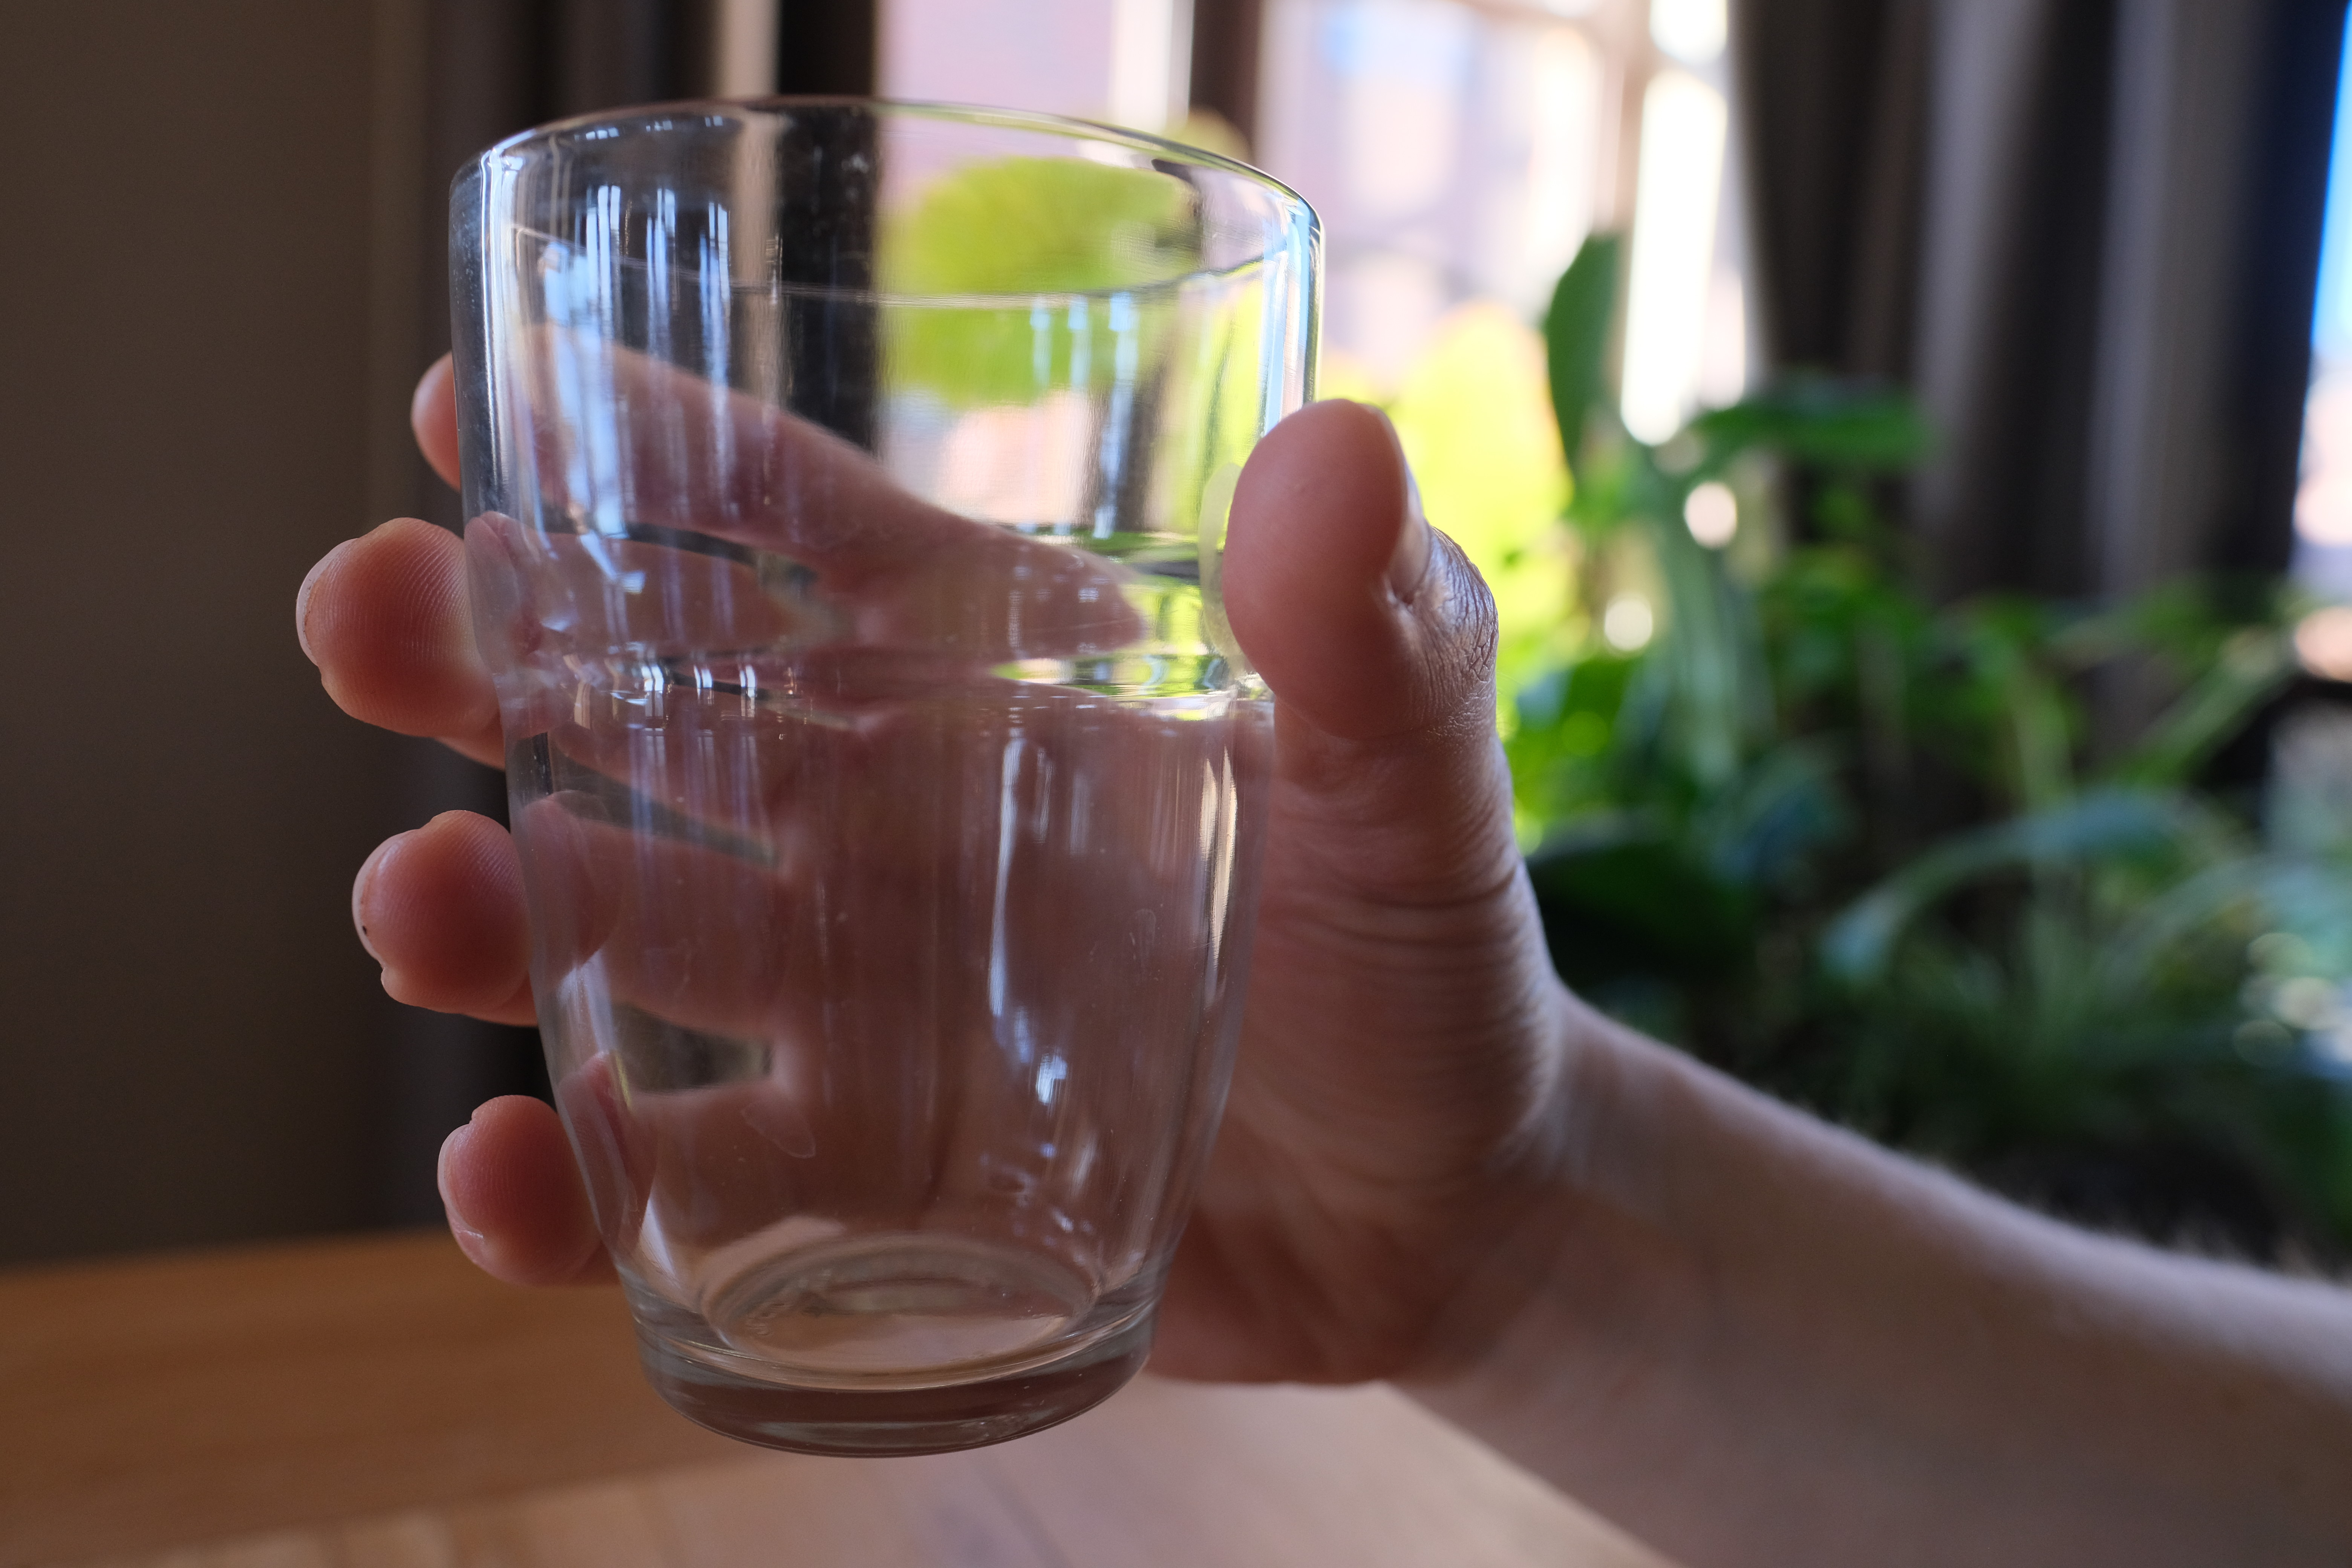
\includegraphics[keepaspectratio, width=\textwidth]{figures/fig_glass.jpg}
        \caption{}
        \label{fig:force_closure_deform_object_glass}
    \end{subfigure}
    \par\medskip
    \begin{subfigure}[b]{0.95\textwidth}
        \centering
        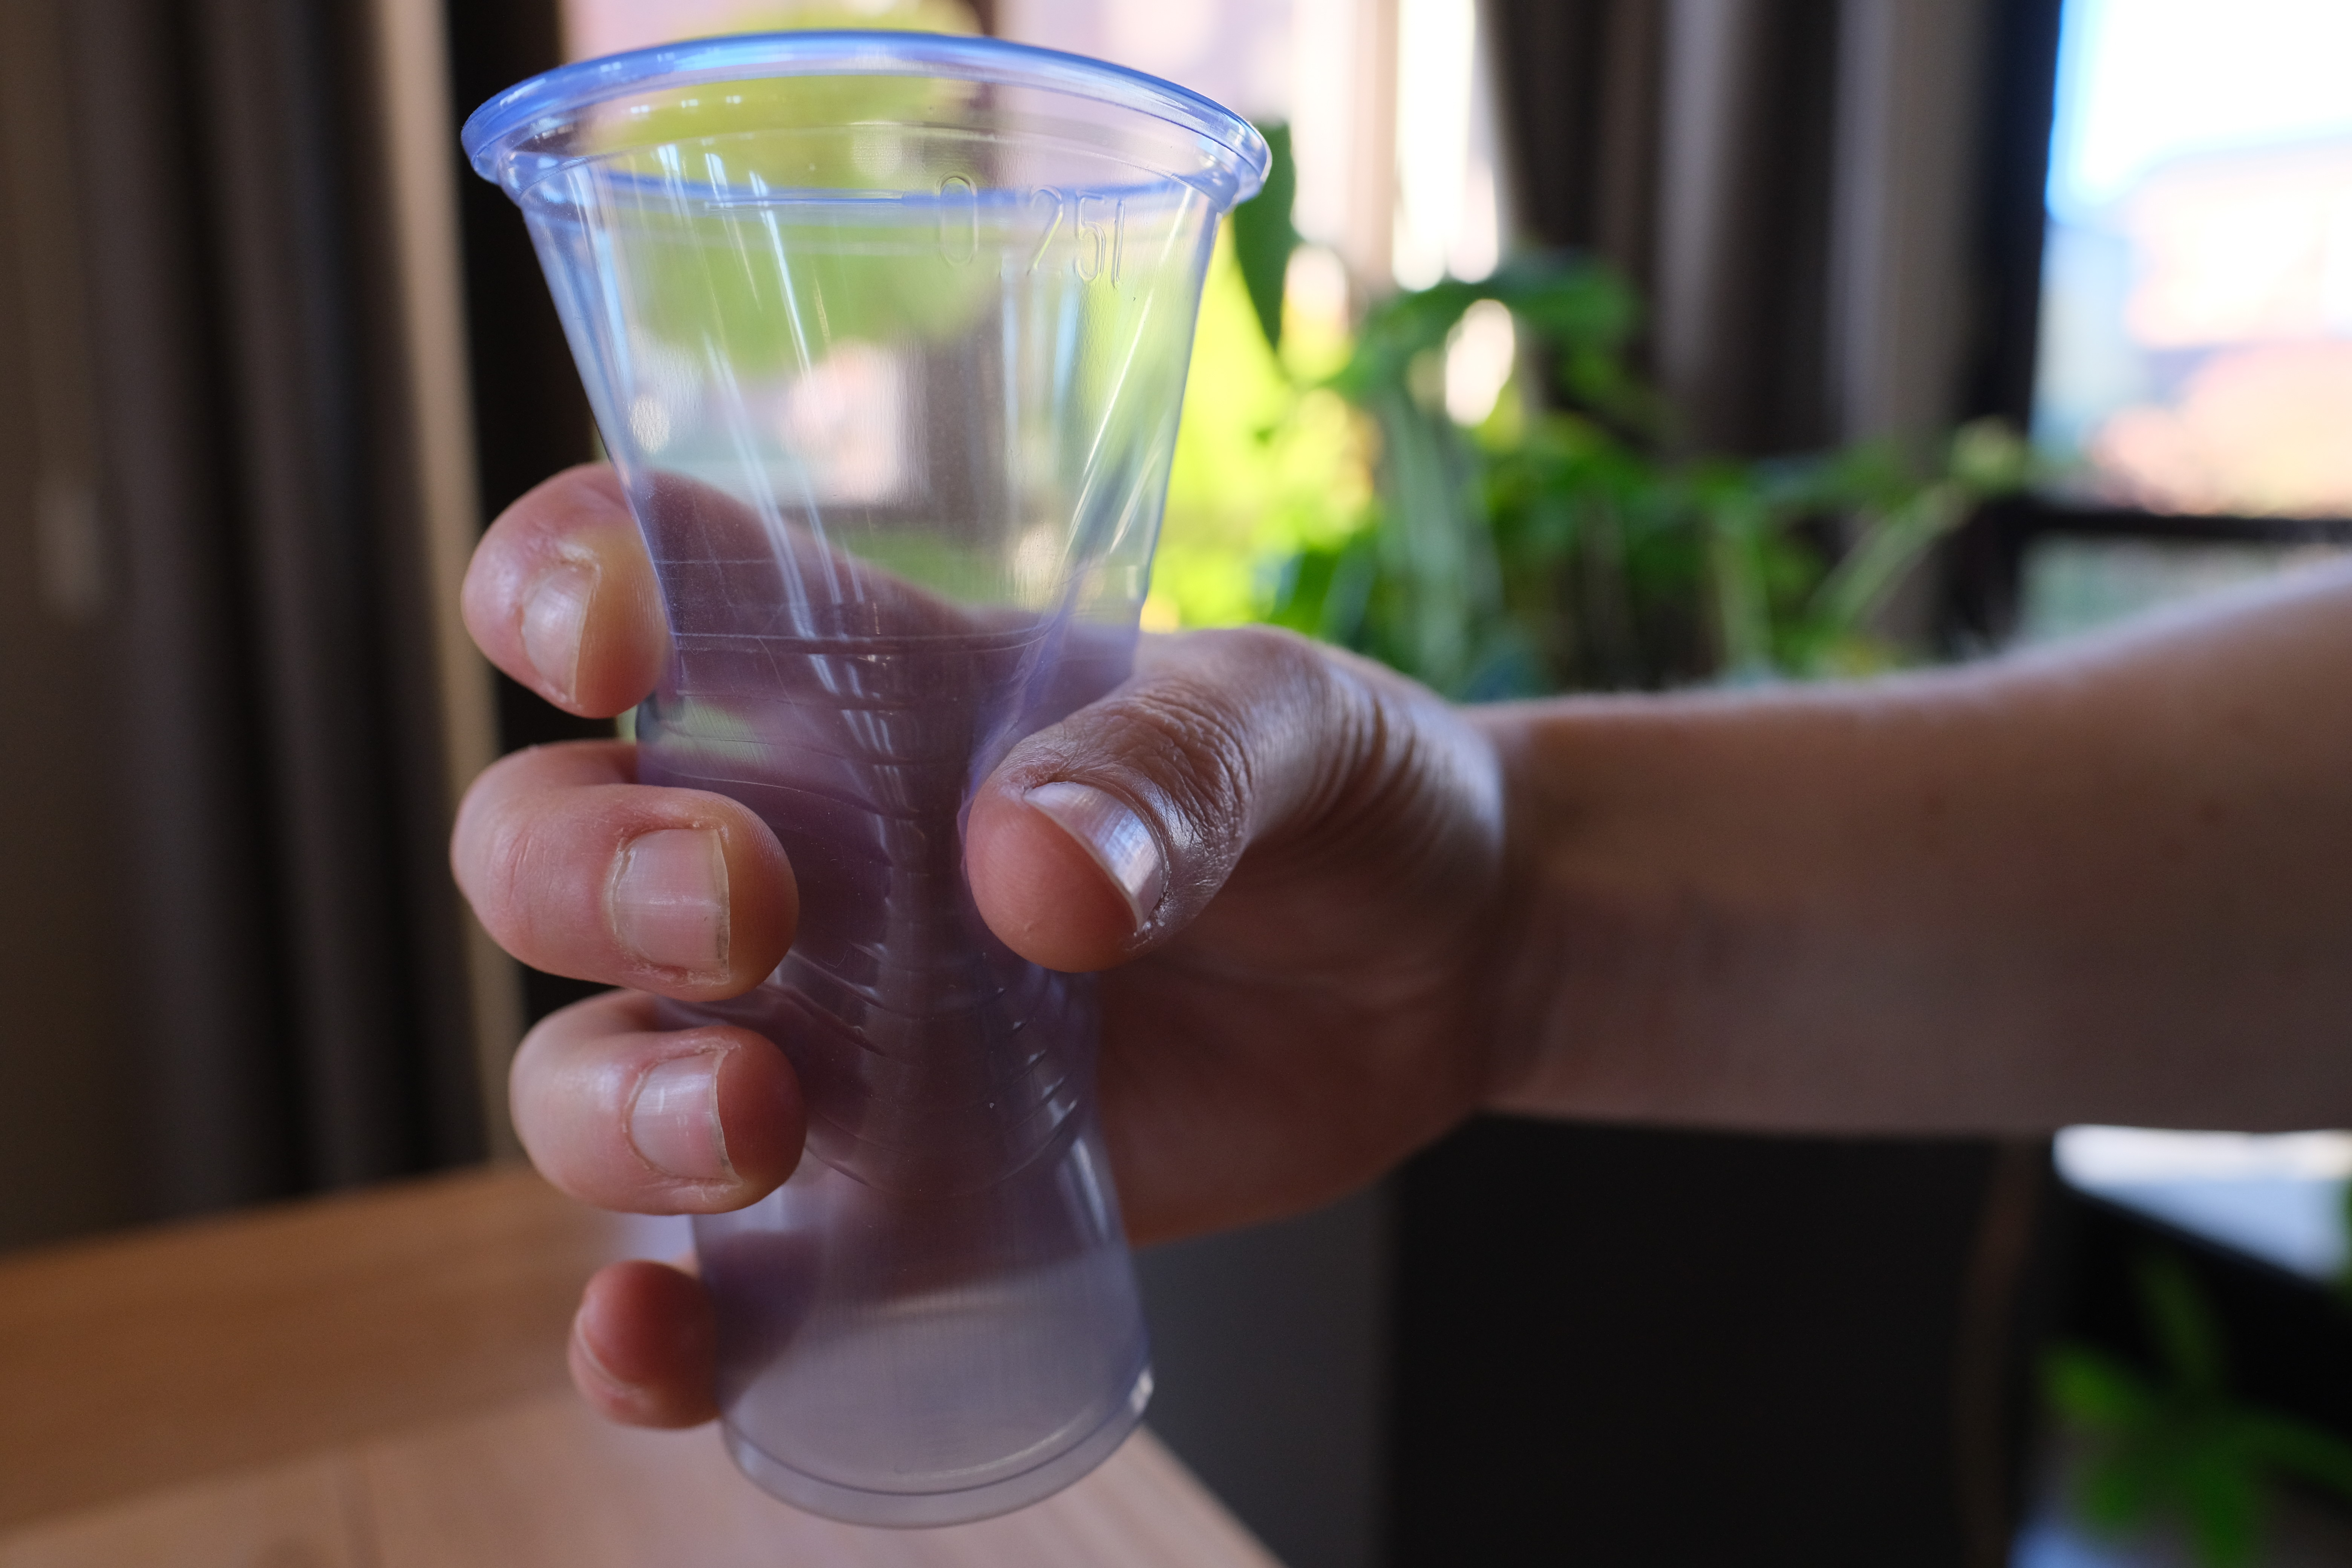
\includegraphics[keepaspectratio, width=\textwidth]{figures/fig_cup.JPG}
        \caption{}
        \label{fig:force_closure_deform_object_cup}
    \end{subfigure}

    \caption[Force closure examples.]{Force closure on a rigid glass (a) and a deformable, plastic cup (b). The deformations of the plastic cup need to be taken into account when calculating a grasping pose.}
    \label{fig:force_closure_deform_object}
\end{figure}

\subsection{Deformable objects: definition, categorization, tasks and solutions}
% Vervormbare objecten: wat zijn ze, categorisatie, welke taken en welke oude pipelines bestaan er
A deformable object is an object whose shape changes when being subject to an external force. This deformation can be temporary and reversible (\textit{elastic}), permanent (\textit{plastic}) or a combination of both (\textit{elasto-plastic}). Deformable objects are found in industrial settings, agriculture and household items. A common categorization \autocite{Saadat2002,Jimenez2012} is based on the geometry of the object: how many dimensions are significantly larger than the other dimensions. The rationale for this categorization is given by small dimensions of the object having a negligible impact on the deformable properties. A canonical example where this property is applied is found in the sheet metal bending industry: the thickness of metal sheets is neglected when computing the required manipulations for bending \autocite{Duflou2005}. A consequence of this categorization is that 3D objects can be considered as 2D deformable objects. For example, both a hollow rubber ball and plush ball can be considered 3D deformable objects based on their dimensionality. However, when considering the dimensions that only impacts the deformable properties, a hollow ball is 2D deformable object as the thickness can be neglected for manipulation. 
\keyWithTitle{Deformable objects}{A deformable object is an object whose shape changes on interaction and can be categorized based on the number of dimensions negligible for manipulation planning.}
In its simplest setting, the deformable object is one dimensional: ropes, strings, cables, threads and catheters, among others. Some of these examples are shown in \cref{fig:dlo_examples}. These objects are also known as deformable linear objects. The term \textit{linear} refers to one dimension being dominant over the other two dimensions. Common tasks for deformable linear objects involve grasping and manipulating ropes, for example, knot tying. Early motor control architectures for solving tasks regarding deformable linear objects used either an open-loop approach or simple visual servoing to execute the motion. An early work clearly demonstrating modular control pipelines is the project of~\citeauthor{Inaba1987} in~\citeyear{Inaba1987}. Their method employs visual servoing for manipulating a rope into a ring and then tying the rope. 
Their perception module uses stereo images to detect the rope and the ring. The planning module is hard-coded to iterate through a set of predefined steps while using the detected centre of the ring and 3D coordinates of the endpoints of the rope from the perception module. An inverse kinematics module provides a target trajectory to the low-level controller. Similar modular pipelines can be found in \autocite{Remde1999} for grasping a rope and in \autocite{Saha2007} where knots are tied with needles using probabilistic trajectories of the rope from a simulated model. Incorporating motion primitives, i.e.\ a predefined set of motor actions corresponding to high-level actions, in the planning module is used in \autocite{Yamakawa2008, Vinh2012} to tie knots in a rope.

\begin{figure}[htbp!]
    \centering
    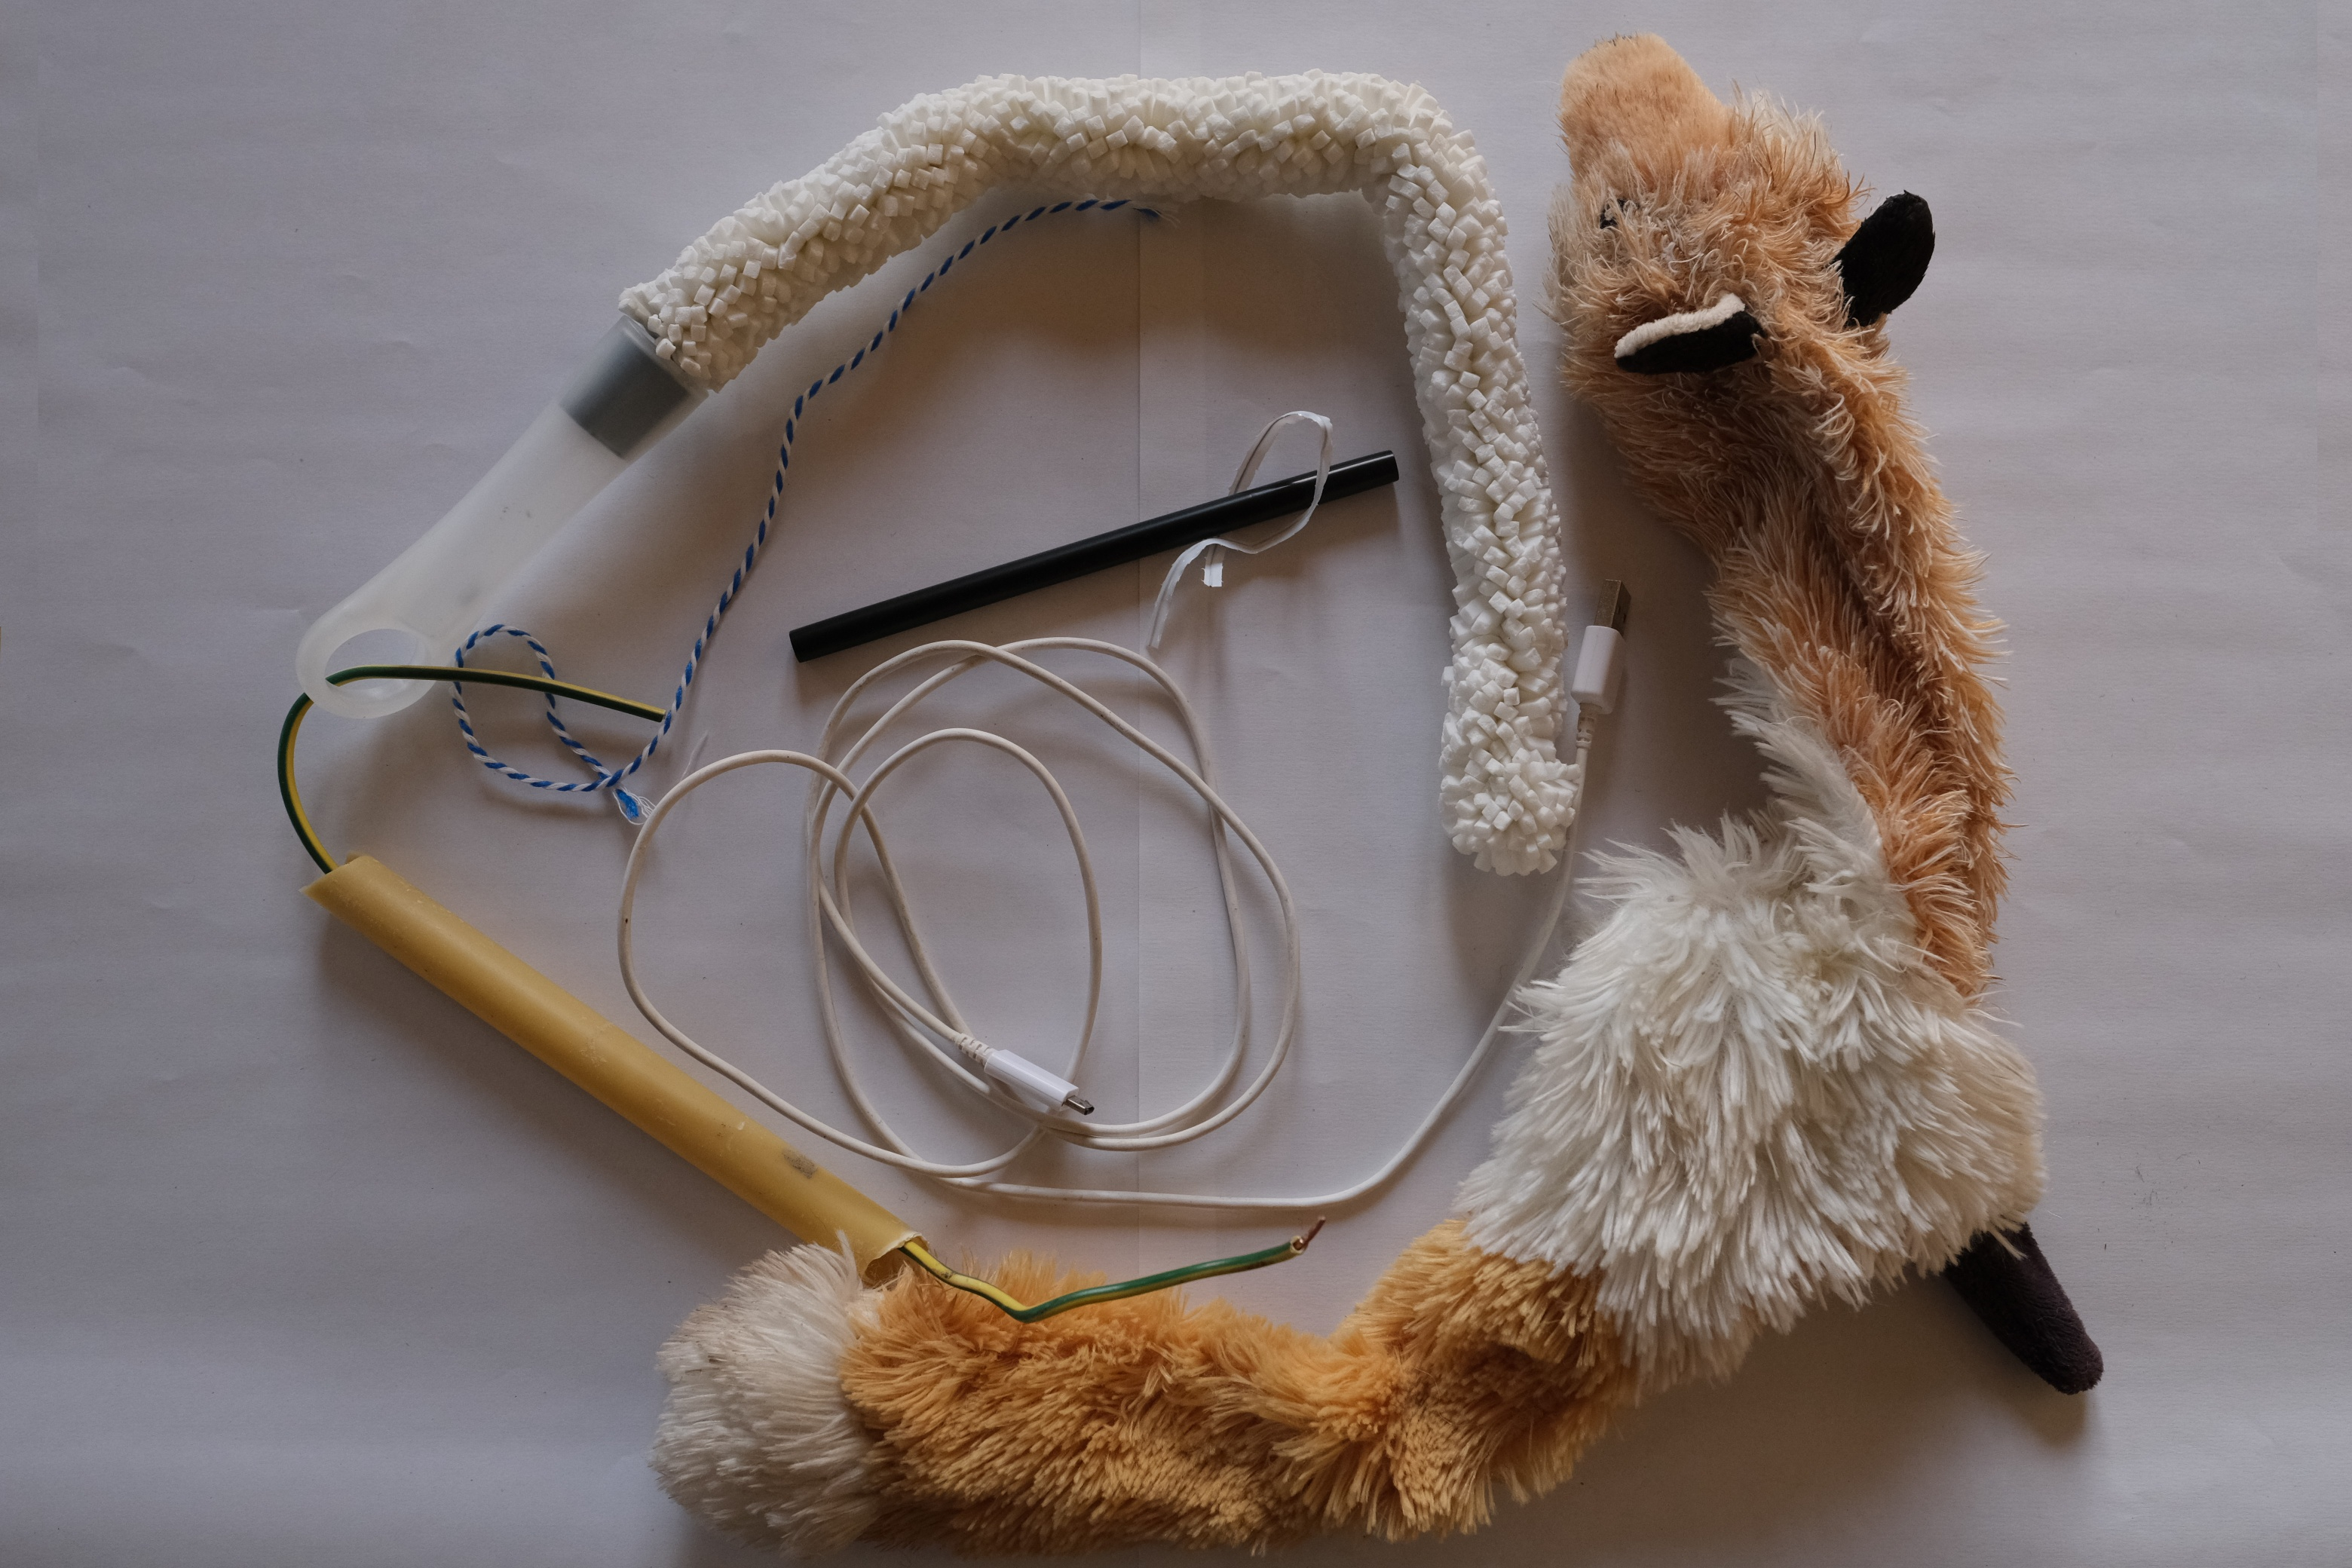
\includegraphics[keepaspectratio,width=\textwidth]{figures/fig_dlos.JPG}
    \caption[Real-life examples of deformable linear objects.]{Examples of deformable linear objects and an application of putting an electrical wire into a rigid pipe.}
    \label{fig:dlo_examples}
\end{figure}

% 2D objects klassieke pipelines
Deformable \textit{linear} objects become deformable \textit{planar} objects when two dimensions are significantly larger than the third dimension. 
In this case, the planning module can disregard the thickness of the material for manipulation. Canonical examples are given in \cref{fig:planar_deform_objects_examples} and contain objects such as clothing, thin-shelled objects like plastic bottles, fabric, paper, and plastic bags, deformable sheets, cards and foam materials. A classic example of paper folding is robotic origami, in which a robot has to sculpt a piece of paper into the desired shape by folding. This problem was tackled with an open-loop control architecture in \autocite{Balkcom2008} to produce a folded hat. \Textcite{Elbrechter2012} takes this a step further by using vision, simulation and fiducial markers on the paper to grasp and fold a paper with a five-fingered end-effector. Related to origami is carton folding and metal sheet bending. Typical control strategies \autocite{Liang1999,Liu2003,Aomura2002} consist of finding the correct locations and sequence of bending operations by modelling the object as a collection of panes articulated through hinge joints. Robotic manipulation of bags has been less studied due to the complexity of modelling and manipulating bags. To circumvent this complexity, dedicated hardware has been researched for grasping \autocite{Kazerooni2005} and unloading \autocite{Kirchheim2008} sacks. A general-purpose two-fingered robotic gripper is used in \autocite{Klingbeil2011} to grasp objects from a table, search the barcode and drop the object into a bag. The planner uses 3D points clouds of depth images taken by a camera. However, they assume the bag is already open for insertion and do not consider any possible deformations caused by touching or dropping an item into the bag.

In the context of this research, it is of interest to note that garments satisfy the same geometrical property of having one negligible dimension as objects such as paper and plastic bottles. However, the main characteristic distinguishing cloth is the compression strength: compared to other two-dimensional deformable objects, cloth does not possess any significant compression strength. Given that the current work deals with manipulations of clothing items, we dedicate \cref{sec:lit_cloth_folding_pipelines} to elaborate on cloth manipulation pipelines.

\begin{figure}[htbp!]
    \centering
    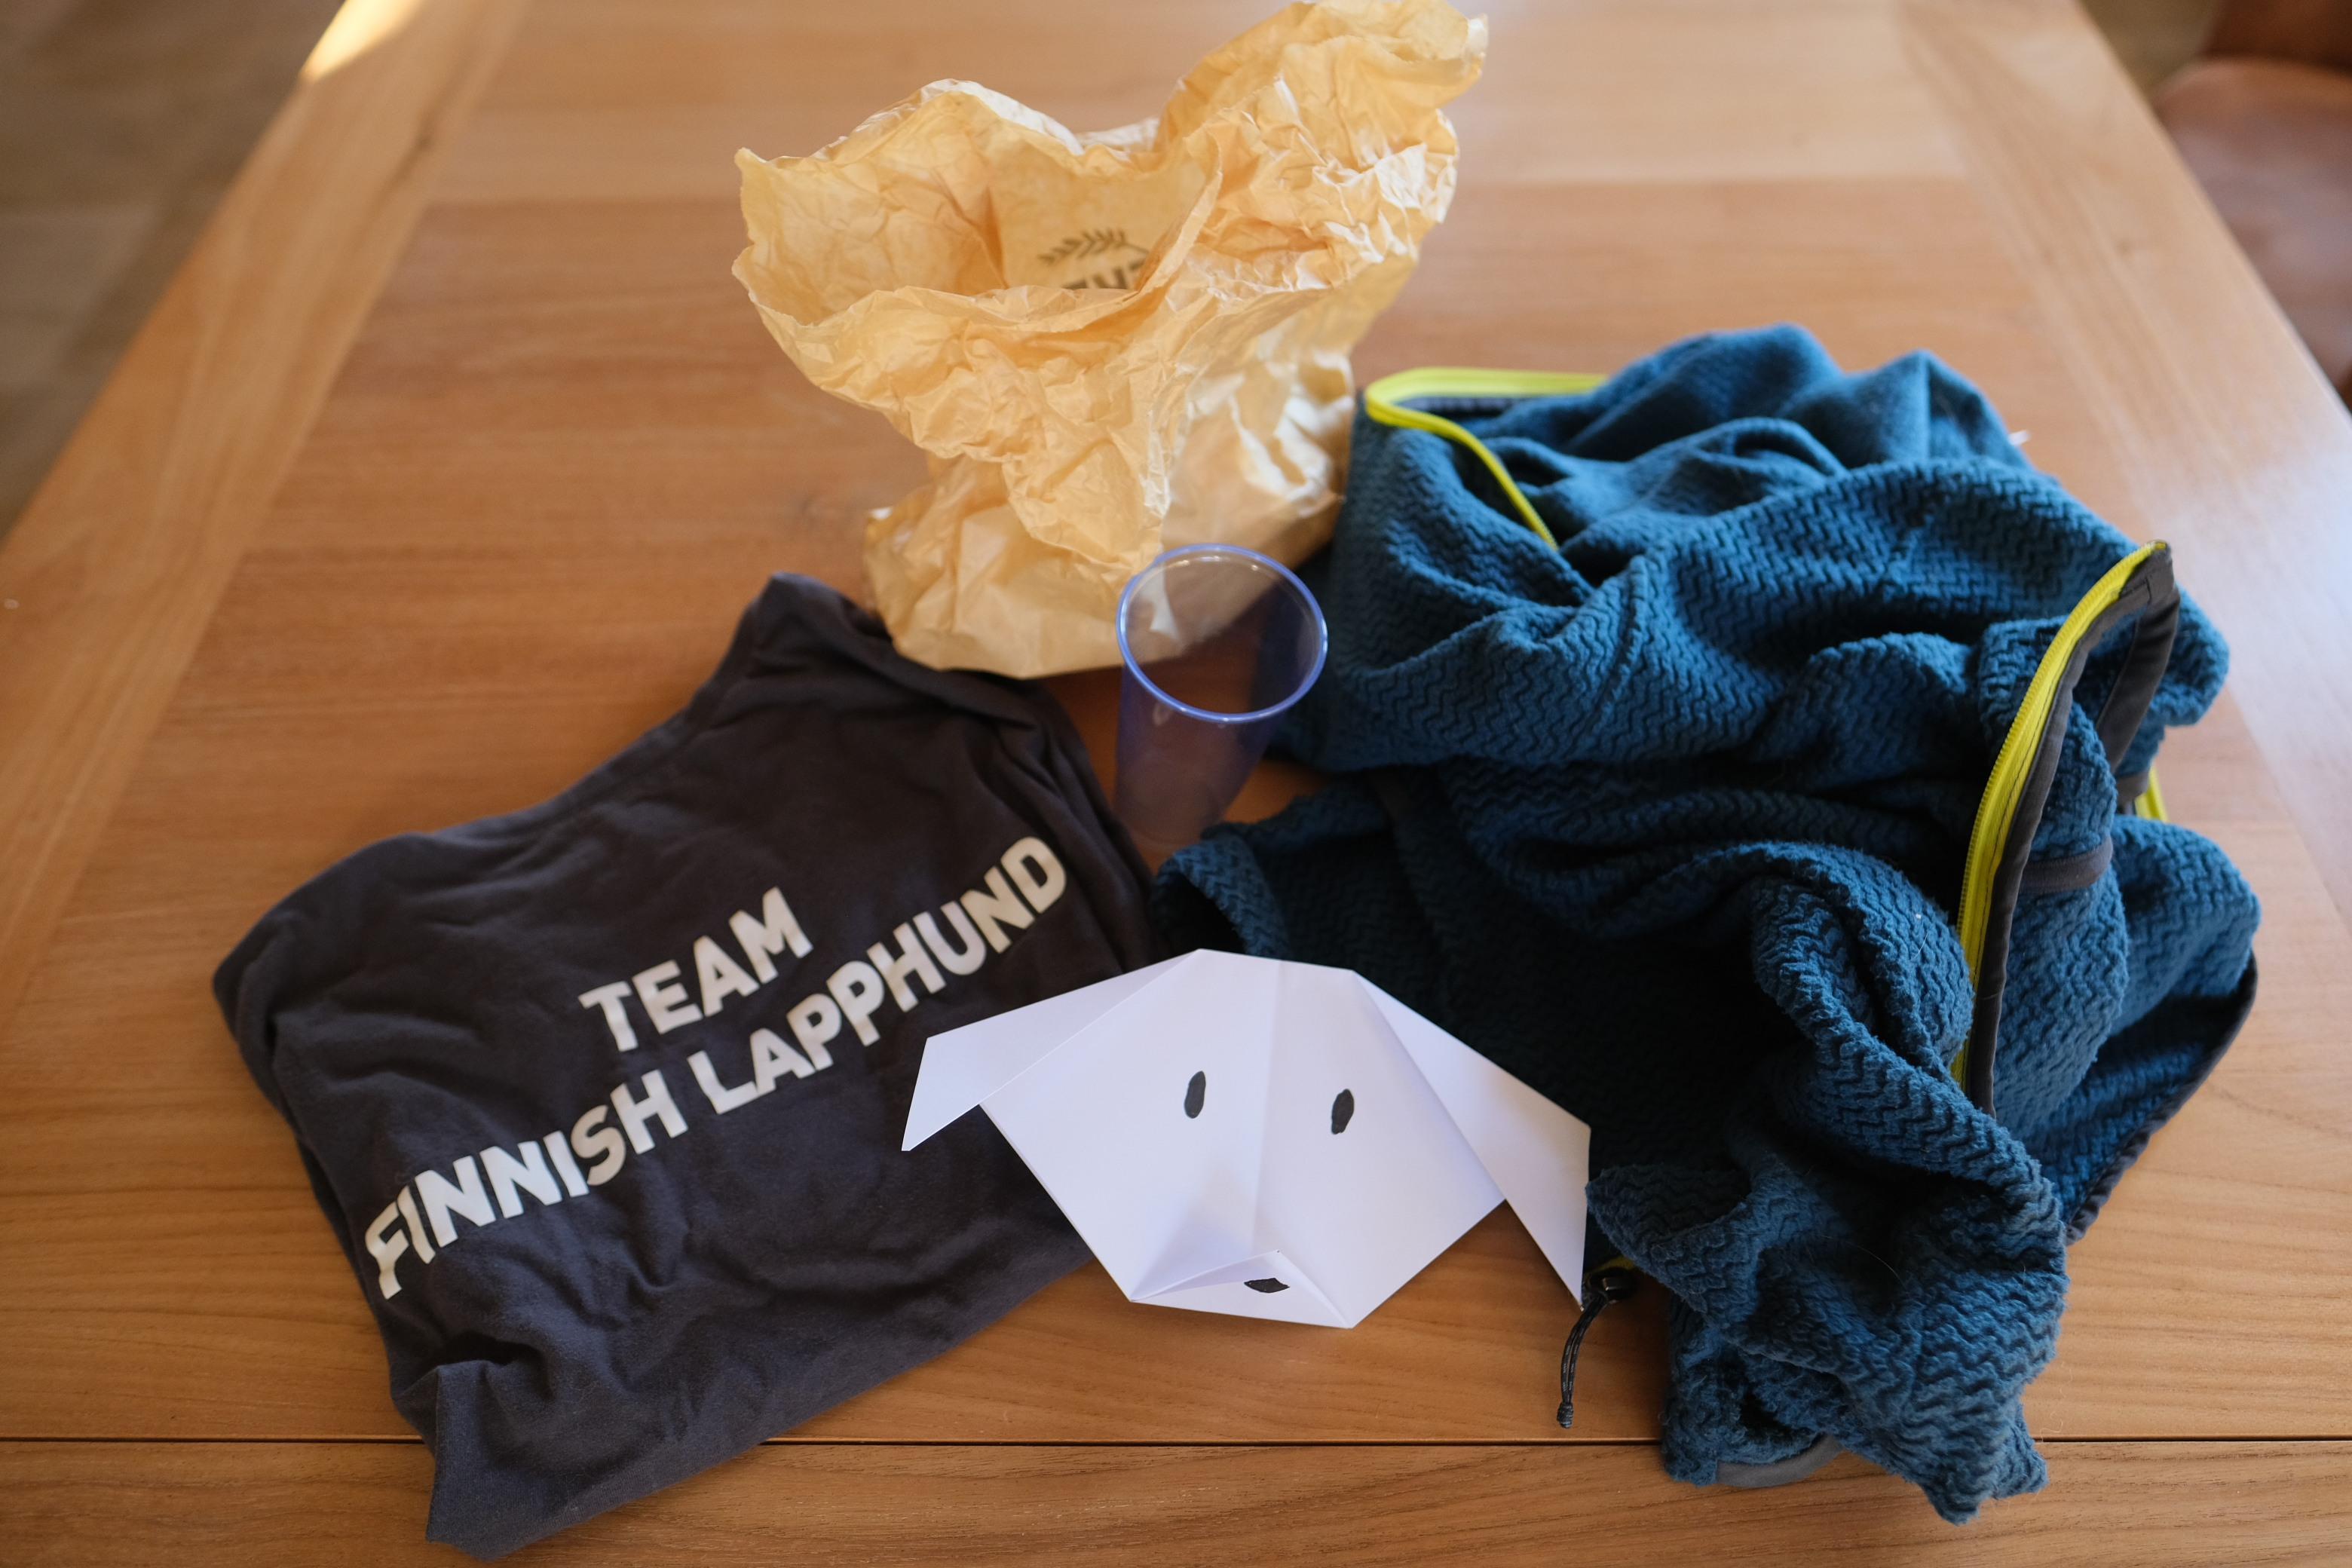
\includegraphics[keepaspectratio,width=\textwidth]{figures/fig_2d_deformables_ex.JPG}
    \caption[Examples of 2D deformable objects]{Examples of 2D deformable objects: origami, paper bag, shirt, jumper and a cup.}
    \label{fig:planar_deform_objects_examples}
\end{figure}

% 3D objects klassieke pipelines
The final category of deformable objects is \textit{volumetric deformable objects} whose deformations across all dimensions of the object are of relevance. Some examples are shown in \cref{fig:volumetric_deform_objects_examples}: objects such as food, plush toys and sponges. In the case of food products, deformations can be caused by both grasping and processing operations such as slicing. In general, 3D deformable objects are the least researched type of deformable objects \autocite{Sanchez2018}. An exception to this is soft tissue, which is important for medical application. We refer the reader to the review paper by \textcite{Taylor2016} for an overview of medical robots in surgery applications. An overview of robotic manipulation of food products is given in \textcite{Chua2003}.

\begin{figure}[htbp!]
    \centering
    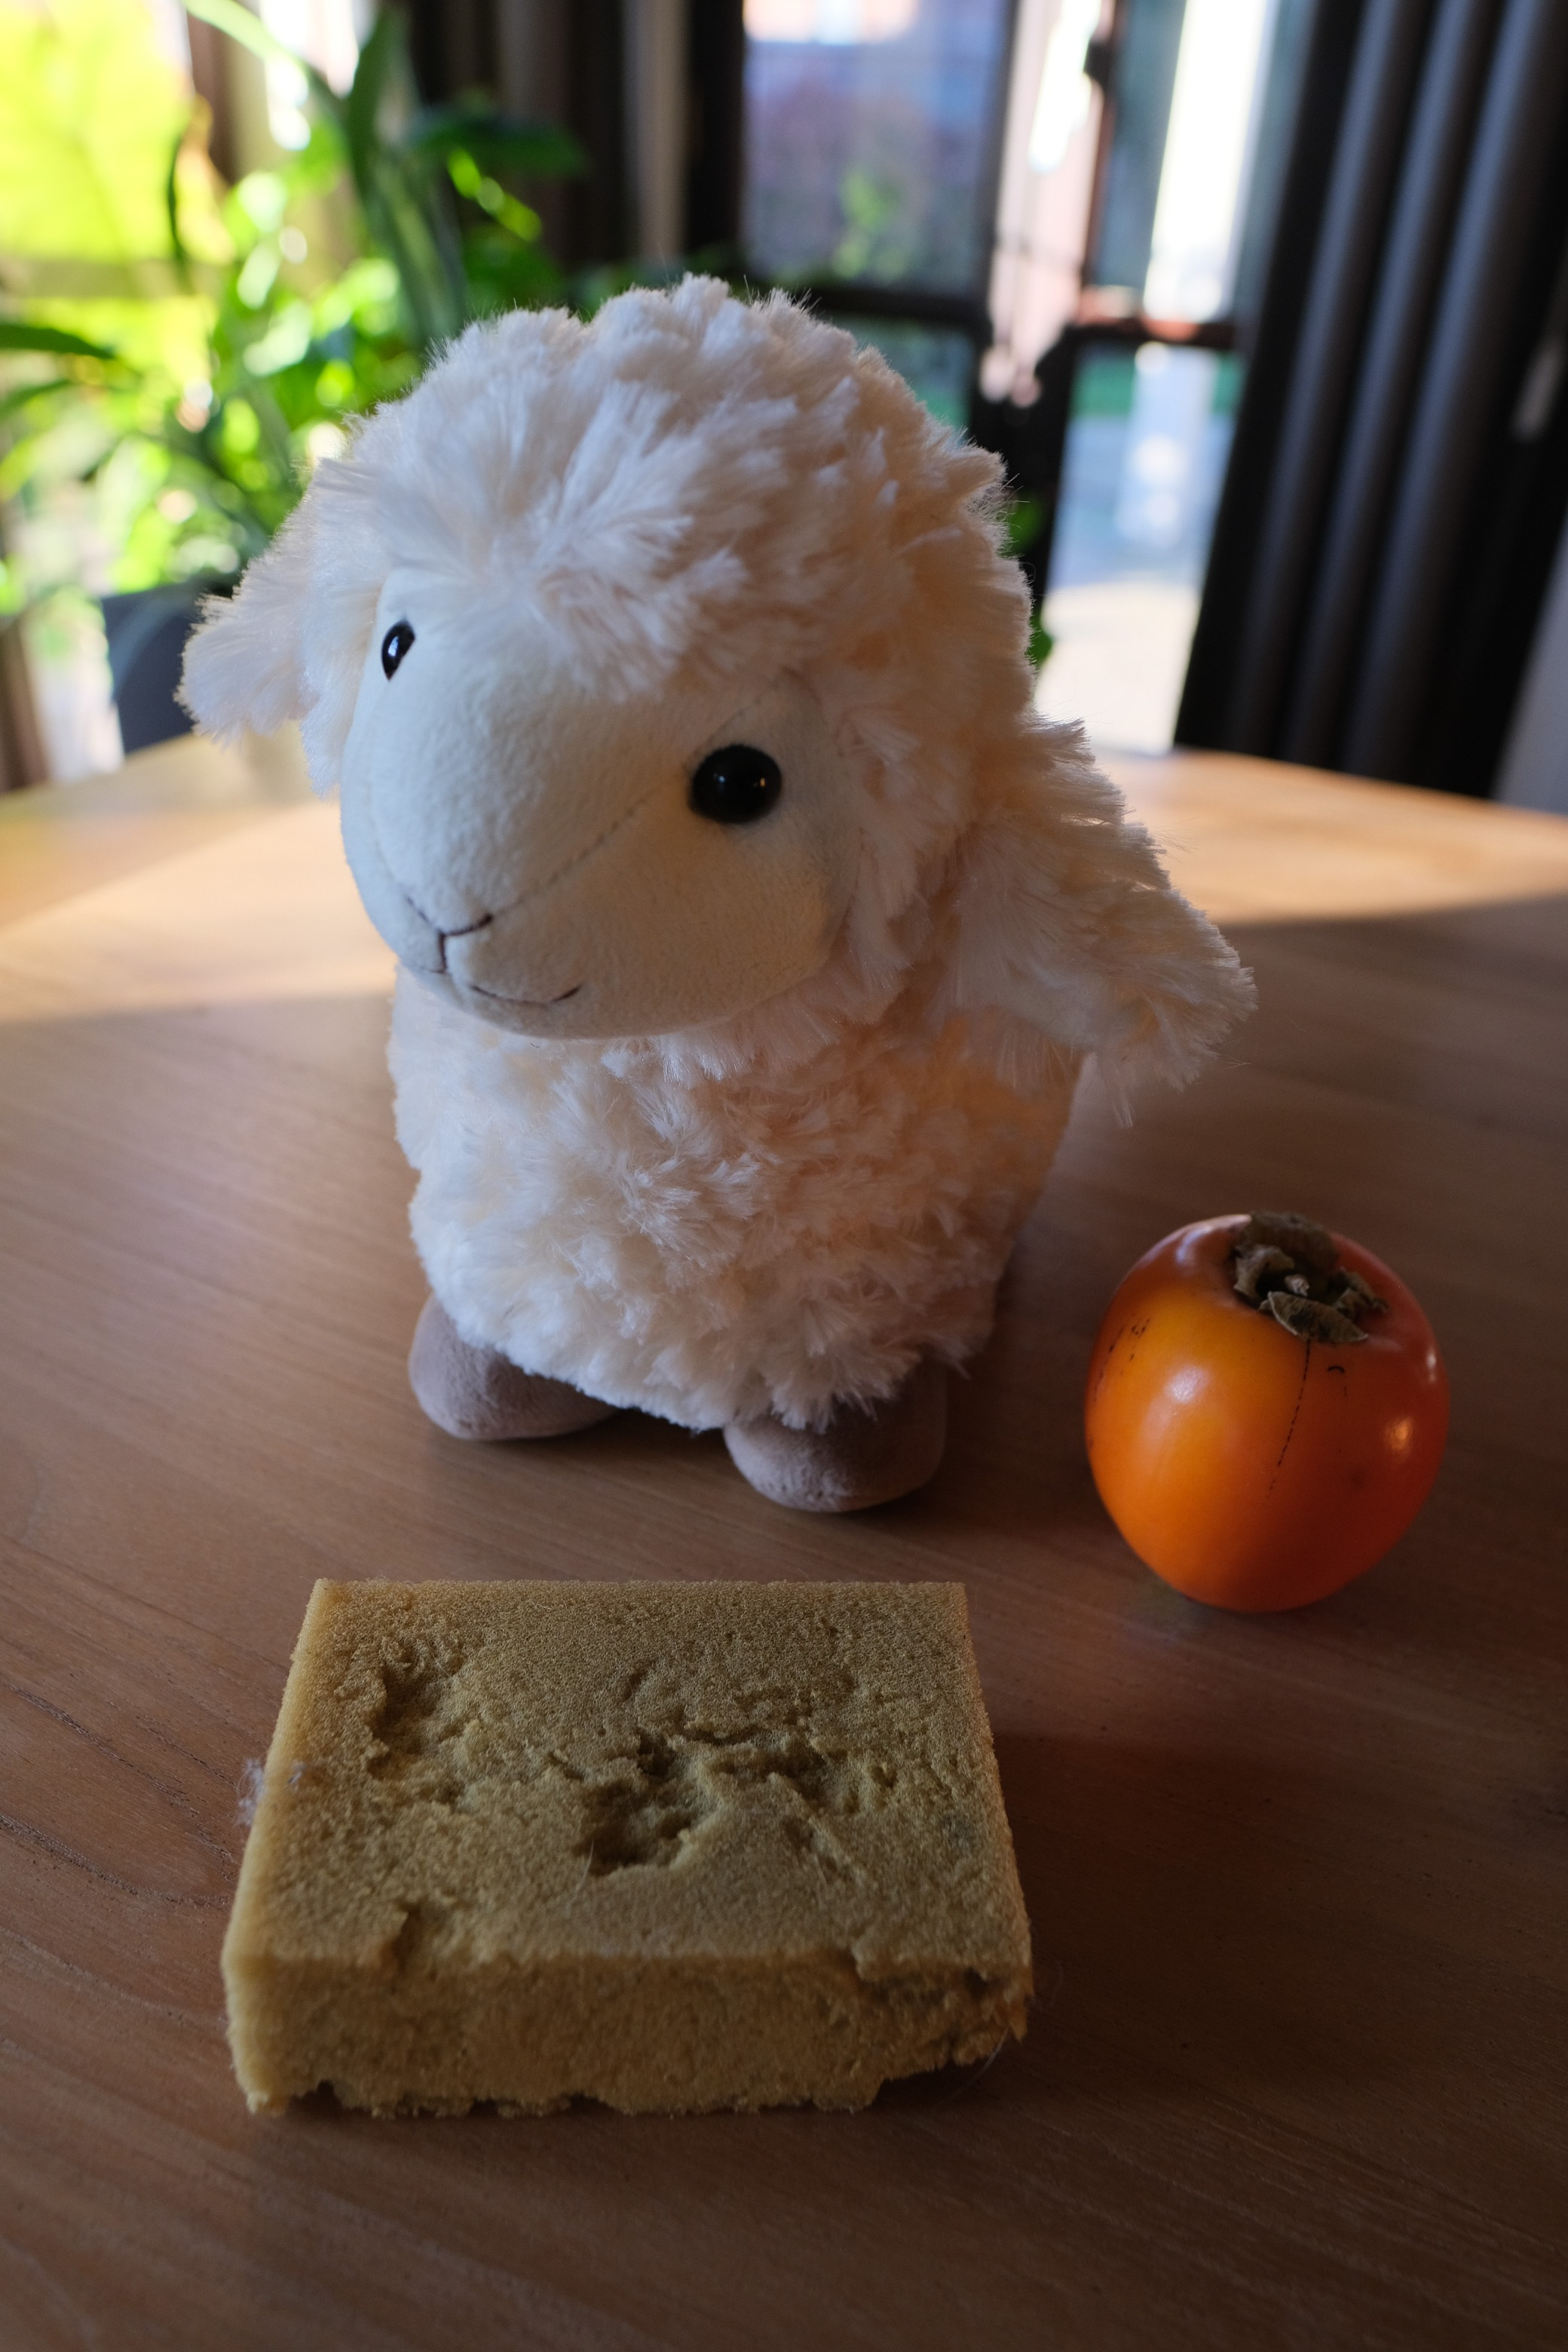
\includegraphics[keepaspectratio,width=\textwidth]{figures/fig_3d_deformables_ex.JPG}
    \caption[Solid deformable objects]{Examples of volumetric deformable objects: sponge, fruit and plush toy}
    \label{fig:volumetric_deform_objects_examples}
\end{figure}
\section{Engineered cloth folding pipelines} \label{sec:lit_cloth_folding_pipelines}
%  wat is het doel van deze subsectie?  = Inzicht verschaffen in hoe "klassieke" pipelines het probleem opdelen (is al geschreven :)) en hoe ze die problemen typisch aanpakken. Doel is dat lezer hieruit kan afleiden dat dat wel cool is maar: traag, error accumulation, geen knowledge reuse etc. 
A high-level categorization of cloth tasks are \emph{sensing} of material properties, \emph{grasping} a single clothing item in a clutter environment and task-specific \emph{manipulation} applications. Specific applications dealing with manipulation of cloth are folding clothing items, hanging cloth on a rod and bedsheet folding among others. In this dissertation, we focus on the application of cloth folding. A complete cloth folding pipeline is visualized in \cref{fig:complete_folding_pipeline}. This folding pipeline typically consists of the following subtasks: (1) grasping an isolated garment, (2) bringing it into a folded configuration and (3) stacking it on top of other folded garments. The second step in this process is often subdivided into unfolding, flattening and folding. Most of the work in robotic cloth folding deal with a single subtask instead of providing solutions to the complete pipeline. Two notable exceptions that consider the whole robotic folding pipeline is the work of~\textcite{Doumanoglou2016,Maitin2010}, which is discussed at the end of this section.
% TODO: add figure of robotic folding pipeline
\begin{figure}[htbp!]
    \centering
    \subfile{figures/fig-folding-pipeline-subtasks.tex}
    \caption{Cloth folding pipeline for robotic manipulation with subtasks.}
    \label{fig:complete_folding_pipeline}
\end{figure}

An evident solution for cloth folding is to use specialized hardware in a constrained environment.~\Textcite{Nair2013} propose an actuated flipfold\footnote{A flipfold is a device consisting of four panels joined by hinges. The four panels lineup with the two sleeves, top-center and bottom-center of the shirt respectively. The hinges allow the panels to rotate inwards. This movement takes the cloth with it and as such makes the folds.} that automates folding of shirts. More complex commercially available products exists such as the FoldiMate\footnote{\url{https://foldimate.com/}}. However, such products do not generalize towards general cloth folding, do not leverage general-purpose robotic hardware and have proven difficult to bring commercially available\footnote{FoldiMate has been in prototype development for nine years at time of writing.}. This is why most research consider the use of general-purpose robot arms, possibly with dedicated gripper and instrumentation, as elaborated in Section~\ref{sec:lit_instrumentation}.

Much of the literature around cloth folding has resolved around solving subtasks of the folding pipeline. In the following subsections, we provide a summary of important work concerning each of the subtasks and describe two important works that consider the complete folding pipeline.

\subsection{Grasping}
Grasping a piece of cloth requires isolating a single piece of garment from a pile of clothing articles and making sure that one functional piece is grasped. In~\autocite{Ramisa2012}, this is done by grasping shirts via the collar. Visual servoing is used with preprocessed features on depth data. Their method achieves a grasping success rate of $70\%$. However, the performance drops to $30\%$ when other types of garments are present on the table. ~\autocite{Monso2012} separate all clothing articles with a robot manipulator. Occlusion of clothing articles leads to uncertainty of the state estimation. They model this explicitly by training a \acrshort{POMDP} for the cloth state estimation.

\subsection{Pose estimation}
After grasping a clothing article, pose estimation is usually done such that the type and configuration of the cloth can be brought into an unfolded state, ready for folding. Garment pose estimation has been done by matching video images to simulation models~\autocite{Kita2002}, using machine learning models~\autocite{Li2014, li2014volum} or instrumentation via fiducial markers~\autocite{Bersch2011}.

\subsection{Unfolding}
Unfolding is an important step as it allows to bring the article into a known configuration from which predefined folding strategies can be employed. A general approach to unfold clothing articles is to exploit gravity; by grasping the article at strategic points, gravity will remove arbitrary folds. \Textcite{Hamajima1998} exploit this gravitational trick by regrasping the hemlines of the garments. The hemlines are detected using the shadows and shape of the cloth. \textcite{Cusumano2011} unfolds shirts and trousers in a two-staged pipeline using \acrshortpl{HMM}, a cloth simulator and a planning algorithm. By inputting the clothing article type, size and grasping points for the gripper to the \acrshort{HMM}, it can estimate the garment's configuration. This configuration is used by the simulation model to find the minimum-energy configuration. This is the configuration in which the garments triangulated mesh vertices have minimum gravitational potential energy. Then, the planning module repeatedly executes trajectories to regrasp the clothing article until it is in a known configuration. Then, the planning module brings the garment into the hard-coded, unfolded configuration. Their method achieves a $66\%$ success rate. \textcite{Doumanoglou2014} solves the same task but reduces the amount of software modules by repeatedly regrasping the lowest hanging point of the garment. This brings the clothing item into a known configuration. Next, the robot unfolds the article by searching two grasping points using a \acrshort{POMDP}.

\subsection{Flattening}
Before folding the cloth into the desired configuration, it is necessary to remove wrinkles caused by unfolding the cloth. Moreover, folding often relies on template matching which is made more difficult when there are wrinkles present. A dedicated method for cloth flattening is proposed in \autocite{Sun2015}. Their method assumes the clothing item is unfolded on a table. They employ RGB-D data to find wrinkles and represent them as fifth-order polynomials. The largest wrinkle is then flattened by using preprogrammed motions of the arms. In \autocite{Willimon2011}, a washcloth is flattened in two phases. In the first phase, they iteratively pull the cloth away from or towards its centroid to remove minor wrinkles. The second phase utilizes depth information to determine regions of interests with high degree of wrinkles and the necessary direction for removing them.

\subsection{Folding}
\Textcite{Bersch2011} execute an open-loop motor control trajectory to fold clothing after unfolding it using fiducial markers on the cloth. The folding loop exhibits a common human strategy to fold cloth: grasp the garment by the shoulders, rotate the sleeves inwards and fold the shirt inwards while placing it on the table. In~\autocite{Berg2010}, they employ a geometry based folding method which folds over predefined lines. Their method relies on using gravity to immobilize parts of the garment such that parts of the cloth become rigid objects.~\autocite{Miller2012} estimate the pose of the garment by fitting a user-specified polygon representation to the detected cloth contours. Then, they apply the same method as~\autocite{Berg2010} to fold the cloth. \Autocite{Yamakawa2011} start folding a cloth in midair, held by its corners, with an algebraic representation of the cloth. They use this simulation model to estimate the pose of the end-effectors at exact intervals such that open-loop trajectory of the points describes a folded garment. Contrary to previous mentioned approaches which rely on a dual-robot arm platform,~\autocite{Petrik2017} considers folding with a single robotic arm. They compute a trajectory in simulation based on the grasping location and the folding line of the garment. However, the literature concerning folding with a single robotic arm is rather scarce due to its limited applications.

\subsection{Full pipeline}
The first example of a complete cloth folding pipeline is the work of~\textcite{Maitin2010}. The task starts from an unorganized pile of crumbled towels and ends when all articles are stacked in folded configuration on top of each other. Given that the end of their pipeline consists of executing predefined trajectories, much of their method rely on predecessor steps to bring the clothing into an exactly known configuration. Their method start with color segmentation on the image to select the central clothing article. Next, the grasped towel is rotated and regrasped in order to find and grasp the corners visually. Unfolding is done by shaking and twisting, and pulling the towel taut. Finally, they run a predefined, open-loop trajectory to lay down the unfolded towel on the table and fold it. The pipeline takes $24$ minutes to execute with the grasp point detection phase being the largest bottleneck.

The second full robotic cloth folding implementation is engineered by~\textcite{Doumanoglou2016}. Their setup considers folding a pile of shirts, towels and trousers. By segmenting an image from the pile on color, an isolated piece is grasped. By repeatedly regrasping the lowest hanging point of the garment, they reduce the amount of possible cloth configuration to classify the garment shape using random forests~\autocite{Breiman2001}. The unfolding procedure is equivalent to~\autocite{Maitin2010} and requires a garment classifier, grasp point detector, and a pose estimation module. Flattening the shirt is done using a brush tool on a dedicated cloth folding gripper. Wrinkles are detected by comparing the contours with existing polygonal models of flattened cloths. Finally, the fold is executed by polygon matching of the contours to predefined templates. Their system achieves a throughput of six minutes per garment with $79\%$ success rate. The slowest step in their pipeline is the detection of the desired grasping points for unfolding.

As concluding remark of this section, we observe a reoccurring theme: a divide-and-conquer methodology leads to a loss of information between the different stages, resulting in the accumulation of errors. For example,~\textcite{Doumanoglou2016} report difficulties when folding towels because the perception system labels them as shirts. These individual components are built in a laboratory environment with certain assumptions which are likely to be violated in an unstructured, complex environment. Inaccurate sensor readings together with deformation of the robot’s links also deteriorate the accuracy of these systems. In order for robots to be useful in unstructured environments with complex dynamics, there is a need for controllers that are able to perform robust grasp synthesis when faced with unseen conditions.



% \section{Learning-based approaches to robotic manipulation} \label{sec:lit_learning}

\section{Learning robotic manipulation tasks with labels} \label{subsec:lit_sl}
Machine learning, a domain of artificial intelligence, is the study of algorithms that give computers the ability to learn from and make predictions based on data. For robotics, learning provides a way to deal with the inherent systematic and random errors in robotic systems and variability in unstructured environments. This is because in learning, you optimize for the grasping task, which implicitly adapts the behaviour to imperfections in the system, such as inaccurate sensor readings.

In the following sections, we provide a short review of the fundamentals of relevant machine learning techniques. We discuss learning with and without labels and by trial-and-error. We discuss their relevant applications in robotic manipulation with a focus on the manipulation of deformable objects. 

\subsection{Supervised learning}

Supervised learning is a machine learning paradigm that operates under the setting where there is a set of \textit{input} variables, for example image pixels, that exert influence over other \textit{output} variables, for example whether there is a shirt or trouser in the image.
\keyWithTitle{Supervised learning}{Supervised learning involves learning a mapping from input data $\vec{x}$ to the output data $\var{y}$, provided by the supervisor.}
The components building up a machine learning system are the dataset, the model, loss function and optimization algorithm. These components are discussed next. 
Formally, we can denote the input data as a set $\set{X}$ consisting of vector $\vec{x}^{(i)} \in \set{X} $ with the superscript $i$ referring to the $i$th observation. In the machine learning domain, this set of predictor variables is called \textit{features}. The set $\set{Y}$ contains the output variables $\var{y}^{(i)} \in \set{Y}$. Concatenating tuples of
$\left\{\left(\vec{x}^{(i)}, \var{y}^{(i)}\right) , i \in 1,\dots,\const{N} \right\}$
, often called \textit{examples}, leads to a dataset which can be used for learning. Central in this learning procedure is the idea of \textit{function approximation} in which a function $f$, parametrized by $\vec{\theta}$, maps an input $\vec{x}^{(i)}$ to its corresponding output $\var{y}^{(i)}$:
\begin{equation*}
	f(\vec{x};\vec{\theta}): \set{X} \mapsto \set{Y}\text{.}
\end{equation*}

This mapping, also called \textit{model} or \textit{hypothesis}, comes in many forms such as linear models, tree-based methods, support vector machines and neural networks\footnote{We refer to~\textcite{Murphy2012, Bishop2006, Hastie2001} for a thorough exposition on supervised learning methods.}.
The goal of the learning procedure then becomes to adjust the parameters $\vec{\theta}$ of the model such that a certain performance measure $\mathcal{P}$ is optimized. This metric, called \textit{loss function} $\mathcal{L}$ in machine learning jargon, is specific to the task and domain in which the learning is taking place. In robotic folding for example, the robot might be presented with a candidate grasping pose $\vec{u}$. The robot then has to predict the probability $\hat{\var{y}} = Q_{\vec{\theta}}(\vec{u}, \vec{x}) = \mathbb{E}\left[ \mathcal{S} | \vec{u}, \vec{x} \right]$ of successfully grasping (success denoted with $S$) a shirt, given some input image $\vec{x}$. Note that this example implies a heavy assumption; the availability of a dataset containing tuples of $ \langle\text{grasping pose}, $ $\text{object configuration},$ $\text{probability of success} \rangle$.
In this situation, one could minimize the negative cross-entropy loss:
\begin{equation*}
	\mathcal{L}=-\var{y}^{(i)} \cdot \log \hat{\var{y}}^{(i)} +\left(1-\var{y}^{(i)}\right) \cdot \log \left(1-\hat{\var{y}}^{(i)}\right),
\end{equation*} with $\hat{\var{y}}^{(i)} = f(\vec{x};\vec{\theta})$ being the predicted output of the model for observation $i$.
The optimization problem then becomes to adjust the parameters $\vec{\theta}$ of the model $f$ using the examples $\left(\vec{x}^{(i)}, \var{y}^{(i)}\right)$:
\begin{equation*}
	\vec{\theta}^{*}=\argmax_{\vec{\theta}} \: \mathbb{E}_{p(S, \vec{u}, \vec{x})}\left[\mathcal{L}\left(S, Q_{\vec{\theta}}(\vec{u})\right)\right].
\end{equation*}
The dominant way for heavy parametrized functions such as neural networks to optimize this objective is to use gradient descent. The gradient expresses the direction of the steepest decrease of the loss function $\mathcal{L}$ with respect to the model parameters $\vec{\theta}$. By iteratively updating the parameters in the opposite direction of the gradient, in the case of a minimization objective, we gradually arrive at a local or global minimum:
\begin{equation} \label{eq:gd_update_rule}
	\theta_{j}:=\theta_{j}-\alpha \frac{\partial}{\partial \theta_{j}} \mathcal{L}(\vec{\theta}).
\end{equation}
$\alpha$ determines how large steps we take towards the estimated direction of the closest local minimum. Adaptive methods such as Adam \autocite{Kingma2014} allows taking variable step sizes per variable based on the historical directions of the gradient. Gradient-based optimization methods have proven to be a crucial for training highly parametrized functions such as deep neural networks, which are discussed in the following paragraphs. 

\subsection{Artificial Neural networks} \label{subsubsec:lit_dnn}

% INTRO what is een artificieel neuron tov biologisch neuron
\Glspl{ANN} are the workhorse of modern \gls{AI}. \Glspl{ANN} are loosely inspired by the neural network in a biological brain and the mechanisms of learning in biological organisms. The human brain is build-up by interconnected processing units called neurons. The connection strength between these neurons changes in response to external stimuli. This way, neurons receive, process and send information through the body and brain of biological organisms. Although comparing artificial neural networks to their biological counterpart is criticized as a far-stretch from the inner workings of the human brain, insights and knowledge of the neuroscience field have been useful in designing neural network architectures. The most common computational model of neurons, visualized in \cref{fig:neuron}, simulates biological neurons as a node consisting of inputs, weights, bias, activation function and an output value. An \gls{ANN} computes an output by propagating the computed values from the input neurons to the output neurons. The artificial neurons are connected through weights that scale the given input to the neuron. A single neuron performs a weighted sum of the inputs in order to arrive at the neuron's \textit{activation}. Next, it transforms the activation value through an activation function before passing it to the successor neurons. The neuron's activation function is the source of nonlinearity in the network and enables the handling of non-linear relationships between inputs and outputs.

\begin{figure}[htbp]
	\centering
	\subfile{figures/fig-neuron.tex}
	\caption[Computational model of a single neuron.]{\textbf{ Computational model of a single neuron.} $x_0, x_1, x_2$ represent input examples or signals from other units within the network. The bias term $b$ represents an external input to the unit. The activation function is denoted by $f$ and applied on the weighted input entering the unit.}
	\label{fig:neuron}
\end{figure}

% Wiskunde neuron
More formally, the output $y$ of an artificial neuron is computed by
\begin{equation}\label{eq:neuron}
	y = f\left(b + \sum_{n = 1}^{D} w_i x_i \right)\,,
\end{equation}
where $f$ is the activation function, $b$ is the bias, $x_i$ is the $i$th input of the neuron which is weighted by weight $w_i$ connecting the $i$th input. An example of an activation function $f$ is the \gls{RELU}~\autocite{glorot2011deep} activation $f(x) = \max(0, x)$. Other common activation functions are sigmoid, hyperbolic tangents or variations of \glspl{RELU}.

\begin{figure}[htbp]
	\centering
	\subfile{figures/three-layered-mlp.tex}
	\caption[A three-layered, feedforward, fully-connected neural network.]{\textbf{A three-layered, feedforward, fully-connected neural network.} This particular network contains three inputs, two hidden layers and one output layer. All neurons of successive layers are interconnected but there are no connections within in a layer. The inputs are propagated from front to back.}
	\label{fig:three-layer-nn}
\end{figure}

% Neuron in networks: ANN 
In order to perform computations with neurons, we organize them in sequential layers. This gives rise to the name of artificial neural \textit{networks} as they chain together many different functions in a directed acyclic graph. In fully-connected feedforward networks the input and output layer are separated by so-called \textit{hidden layers}. The length of this chain is called the \emph{depth} of the network. This architecture is visualized in \cref{fig:three-layer-nn}. The name of the layer often denotes the operation performed by the layer. For example, a softmax layer performs a \emph{softmax} operation: normalize an input vector of real numbers to probability distribution proportional to the exponentials in the input numbers. Feedforward architectures propagate the inputs sequentially from layer to layer with neurons performing calculations as given in \cref{eq:neuron} but in a vectorized way:
\begin{equation} \label{eq:neuron_output_vectorized}
	\vec{x}^{(k)}=f\left(\vec{b}^{(k)} + \mat{W}^{(k)} \vec{x}^{(k-1)}\right).
\end{equation}
In this \cref{eq:neuron_output_vectorized}, the vector $\vec{x}^{(k)}$ contains the outputs of all neurons in layer $k$ which is based on the input vector $\vec{x}^{(k-1)}$ from previous layer, multiplied with weight matrix $\mat{W}^{(k)}$. The computation occurring in the hidden layers solve a major problem in real-world problems where many applications require disentangling sources of variation by using high-level abstract features. Learned representation offer a solution for such problems because it often results in much better performance compared to hand-designed features. Stacking multiple hidden layers in a neural network allows learning representations based on raw data which solves this central problem of finding features at appropriate levels of abstraction. This paradigm of stacking layers of computational units is called deep learning. It takes a compositional learning approach: upstream representations are expressed in terms of other, simpler downstream representations. Early layers learn primitives which are combined later to form more complex features. In images for example, downstream neurons learn edges and corners which are used in upstream layers to learn to recognize for example the sleeve of a shirt.

% How do we train NNs?
Crucial in neural networks is that the representations are learned instead of crafted by hand. Learning in neural networks occurs by changing the strength of neurons' connections. The weight adjustment is a response to the network's error and has as goal to modify the computation to make the output maximize the given objective. Training of these network weights is done using gradient-based optimization as discussed in \cref{subsec:lit_sl}. Although alternative training methods exist such as evolutionary methods~\autocite{salimans2017evolution}, gradients provide the direction in which to change the weights in order to maximize the objective function. This is especially beneficial for highly parametrized functions such as neural networks. Differentiation of multi-layer neural networks, called backpropagation, was already figured out in~\autocite{rumelhart1986learning} but was rediscovered by running the costly matrix-vector multiplication step in parallel on \gls{GPU}~\autocite{gpu-nn}. Although improved computational hardware and data availability was a crucial enabler of the success of deep learning, many "tweaks" have proven as important to stabilize the backpropagation algorithm. Gradients assume an infinitesimal small step in each direction whereas the actual step we make has a finite length in order to make any real progress in optimization. The problem is that the gradients do change during the course of this step. In the case of multivariable optimization problems of considerable size, which is the case in deep neural networks containing millions of parameters, the optimization landscape is highly non-convex. This treacherous optimization landscape can change the gradients drastically leading to unstable training. This is why gradient-descent strategies such as momentum-based learning, using parameter-specific learning rates and weight initializing schemes are standard tricks in the deep learning practitioners toolkit. Gradients have also been known to disappear and diverge in deep neural networks because of repeated matrix multiplications when propagating the information forward and backward through the network. This is why \gls{RELU} activation functions are popular given that this piecewise linear activation has a derivative of value $1$ in certain intervals and zero elsewhere. Another problem caused by the highly parametrized nature of deep neural networks is overfitting the data. In machine learning jargon, this means that a model can predict the training set well but performs poorly on hold-out samples. A popular way to deal with overfitting is to regularize the network weights. Regularization effectively reduces the network computational power by imposing a penalty on weights in the loss function:
\begin{equation}\label{eq:regularization}
	L(\vec{\theta})=\frac{1}{N} \sum_{n=1}^{N} P\left(f\left(\vec{x}^{(n)}, \vec{\theta}\right), y^{(n)}\right)+\Omega(\vec{\theta}).
\end{equation}
In \cref{eq:regularization}, the function $P(.)$ is a chosen optimization metric that takes the output of the network $f\left(\symbfup{x}^{(n)}, \symbfup{\theta}\right)$ and the real label $y^{(n)}$ of sample $n$ and is domain-dependent. The other term $\Omega(\symbfup{\theta})$ is the regularization term which balances $\ell 1$ and $\ell 2$ norm of the weights:
\begin{equation} \label{eq:regularization-term}
	\Omega(\vec{\theta})=\gamma \underbrace{\sum_{k} \sum_{i} \sum_{j}\left|\mat{W}_{i j}^{(k)}\right|}_{\ell 1 \text { regularization }}+\lambda \underbrace{\sum_{k} \sum_{i} \sum_{j}\left(\mat{W}_{i j}^{(k)}\right)^{2}}_{\ell 2 \text {-regularization }}.
\end{equation}
The hyperparameters $\gamma$ and $\lambda$ in the regularization term of \cref{eq:regularization-term} trade-off the amount of $\ell 1$ and $\ell 2$ regularization. The term $\mat{W}_{i j}^{(k)}$ refers to the weight in layer $k$ connecting neuron $i$ to neuron $j$. $\ell 1$ regularization achieves sparse weights while the $\ell 2$ norm leads to networks with smaller weights. Other popular methods to improve generalization properties of deep neural networks is dropout~\autocite{dropout}, which zeroes out different random neurons at training time, ensembling and using data augmentation.

% CNNs
The feedforward models described above connect the neurons between layers in a fully-connected manner: every neuron from a layer is connected to every neuron from the preceding and succeeding layer with an unique weight. This dense connectivity lead to an explosion in the amount of trainable parameters. However, when the input data contains topological structure, like the ordering of image pixels in a grid, constraining the connectivity pattern between layers is a useful method to reduce the amount of parameters and exploit correlation. The most common way to implement this is by replacing the matrix-vector product $\mat{W}^{(k)} \vec{x}^{(k-1)}$ of \cref{eq:neuron_output_vectorized} with a sum of convolutions. This operation is equivalent to sliding a low-dimensional filter or kernel over the input image while performing a dot product. This property leads to sparse connectivity and parameter sharing. Consequently, by connecting a local spatial region with a shared set of parameters to the full spatial resolution of the image, one imitates the cortical neurons in the visual cortex, which respond only to stimuli within a receptive field~\autocite{hubel1959receptive}. It has been argued that these properties explain the success of using trainable convolutions for computer vision~\autocite{Goodfellow2016}. Usually, the convolution operation is followed by a downsampling operation that provides a summary statistic of the nearby outputs. This is most frequently implemented with an aggregation function, for example max pooling that takes the maximum value of a rectangular neighborhood. The process of embedding convolution operations, optionally followed by pooling operations, is known as a \gls{CNN}. After demonstrating the effectiveness of \glspl{CNN} for large-scale image classification~\autocite{Krizhevsky2012}, \glspl{CNN} have been omnipresent in computer vision and natural language processing. In robotics, convolutional layers can provide a perception module while the motor control module is implemented as fully-connected layers acting on the output of the filter banks. However, in the case of motor control, the pooling operation is ofted removed from the architecture as translational invariance is not a desired property. Invariance to the position of a detected object would not enable a robot to detect where the object is located in the image. For more details about the history and working of deep learning methods and architectures, we refer the reader to the textbook of~\textcite{Goodfellow2016}.


Supervised learning is an important paradigm for robotic learning because labelled data provides a clear learning signal. This is important because time spent on robots is expensive. Contrarily, the learning signal in reinforcement learning (\cref{subsec:lit_rl}) often does not optimize for direct task performance and might lead to expensive learning times on physical robot platforms. The following paragraphs discuss relevant work in applying machine learning methods for solving robotic manipulation tasks. 

\subsection{Supervised learning and neural networks in robotic manipulation research}
% Generally speaking, there are two main strategies for applying supervised learning in the robotic manipulation pipeline: (1) as a perception module or (2) to map states to actions using imitation learning. 
% ---- PERCEPTION MODULE ----- %
% standard ML METHODS
Traditionally, supervised learning methods are leveraged in the \textbf{perception module} of a robotic manipulation pipeline. For rigid body manipulation, the popularity of data-driven grasp synthesis approach took off with the work of~\textcite{Saxena2008}. In their work, a logistic regression classifier is trained on synthetic data using manually engineered features. This way, they demonstrate that a robot is able to unload a dishwasher. In the domain of deformable object manipulation, ~\textcite{Ramisa2012} searches for quality grasping points of crumbled cloth in order to maximize the unfolding upon lifting. They do this by first labelling a dataset of shirts with bounding boxes containing the appropriate grasping points. Next, they train a logistic regression model to obtain the probability of the desired grasping point in a given bounding box using a bag of features from the input image. By employing the logistic classifier in a sliding window over the image, they pass image patches containing local peaks to an \gls{SVM} to obtain more accurate grasping candidates. The candidate patch is converted to 3D space by working in a calibrated environment, and motion planning is executed using inverse kinematics. Similarly,~\textcite{Wang2011} folds socks by having a perception system that uses manually engineered features for training an \gls{SVM} with Gaussian kernel to determine the type of sock in front of the robot. \Glspl{SVM} have also been used for the purpose to identify garment category and pose \autocite{Li2014, li2014volum}.
The deformable nature of cloth leads to self-occlusions making the garment type and pose classification ambiguous. The presence of this hidden state is explicitly modelled using a \gls{HMM} in \autocite{Cusumano2011}.  Learning methods are also being used to find regions of interest on the cloth. For example,~\textcite{Doumanoglou2016} use random forests to learn garment-specific grasping points. In \autocite{Maitin2010}, RANSAC \autocite{RANSAC} is used to find the corners of the cloth. These corners are good candidate grasping points for unfolding and identifying the type of cloth. Finally, nearest neighbours have been used to identify wrinkled regions in a washcloth in order to flatten it \autocite{Willimon2011}.

% NEURAL NETWORKS: supervised learning in perception module
The earliest work using neural networks for deformable object manipulation is \autocite{Howard2000}. In their work, they train a small feedforward neural network that learns the required minimum grasping force for lifting a deformable object. They collect the data by iteratively using more lifting force on objects with certain masses, deformability and damping. 
With the breakthrough in deep learning in~\citeyear{Krizhevsky2012} by~\textcite{Krizhevsky2012}, deep neural networks have found their way into robotic manipulation, starting in the rigid body manipulation domain. A successful approach to training deep neural networks in a supervised setting for robotic manipulation is to use \glspl{CNN} as grasp success predictor.~\textcite{Levine2016} train a \gls{CNN} on a large dataset of $800.000$ grasping attempts to learn to predict the grasp success probability of a grasping pose, given an input image. To sample candidate grasping points, they employ CEM \autocite{CEM}. Dex-Net \autocite{dexnet2} also trains a \gls{CNN} to predict the quality of a grasping candidate. This network is trained using a simulated dataset where objects are put into randomized poses on a plane. They use simulation to evaluate different grasping wrenches using analytic grasp metrics. Their model shows impressive generalizability to the real world, on different models not seen during training. The Dex-Net framework has been extended to work with suction grippers \autocite{dexnet3}, use dual-armed robots \autocite{dexnet4} and generate grasping candidates in the network \autocite{Satish2019}.

% ---- IMITATION LEARNING ----- %
% Standard ML methods
Another strategy to train controllers using supervised learning is \textbf{behavioural cloning}. Behavioural cloning is a type of imitation learning \autocite{Argall2009} in which task demonstrations are used for learning task execution. In behavioural cloning, a sequence of states and actions, as executed by a demonstrator, is recorded as dataset for a supervised learning algorithm. The goal then becomes for the model to predict the action a demonstrator would choose, given a certain state. 
% \todo{Voegen we hier nog een degelijkse uitleg toe wat de verschillende LfD aanpakken zijn? Lijkt me relevant om te weten dat methodes zoals kinesthetic-teach-in niet echt nuttig zijn voor cloth domein.} 
An in-depth view of the field of learning from demonstration is given in \autocite{Argall2009}. In the case of robotic laundry,~\textcite{Jia2019} learns single robotic laundry tasks for flattening, folding and twisting cloth by imitating human examples. Notably in their work is representing the robotic controller using random forests \autocite{Breiman2001} instead of neural networks. The rationale is given by the non-parametric nature of random forests to dynamically change the number of leaf nodes based on the given imitation data and new cloth configurations.
Example demonstrations are also used in deformable object manipulation to tie knots. ~\textcite{Schulman2016learning}, for example, uses example demonstrations for non-rigid warping \autocite{Chui2003} based on point-cloud registration of the scene to tie knots with a robotic manipulator. The general idea is to warp the demonstrated trajectory to match the current setting, which may vary in initial conditions and knot geometry. Closely related is the work in \autocite{Morita2003} where examples and solutions strategies from knot theory is embedded to perform motor control.
% NN for imitation learning
Neural network models have also been a strong candidate for robot learning from demonstration \autocite{Ravichandar2020}. Given the cost associated with real robot rollouts, it is beneficial to lower the dataset requirements by having access to the motor control outputs or to decrease the input dimensionality by for example avoiding learning from pixels. This explains the popularity for teleoperated \autocite{Zhang2018,Duan2017} and kinesthetic teaching \autocite{finn2017one} approaches. However, it is difficult to teleoperate a robot or physically manipulate a robotic arm to fold clothing items. This is because the speed and forces associated while executing the task is relevant for achieving proper folds. One method to compensate for this difficulty is to solve the imitation learning task in simulation and trying to transfer it to the real world. This is explored in \autocite{Seita2020} that generates example demonstrations in simulation and uses behavioral cloning to train a motor policy network to flatten a towel. To fine-tune this policy outside the seen dataset distribution, they employ dataset aggregation (DAgger) in which an oracle policy is used to label the unseen states during training. An alternative is given in \autocite{Sundaresan2020} that uses simulated data to learn visual object descriptors indicating the segments of a rope. Such embeddings implicitly encode geometric structure which can then be used for knot-tying using example demonstrations.
Although imitation learning is a viable alternative for learning to manipulate objects, a general problem plaguing imitation learning methods is generalizing to unseen scenarios. In the case of trajectory execution, errors can accumulate drastically leading to task failures. This is why existing methods apply data augmentation, include teacher advice or use reinforcement learning (\cref{subsec:lit_rl}).

% ---- LEARN DYNAMICS MODEL ----- %
Another approach to leverage the expressiveness of deep neural networks in a supervised setting is to train a \textbf{dynamics model}. This model, often called world model, is obtained by training on $\tuple{\text{state}, \text{action}, \text{next state}}$ tuples. The problem that world models tries to solve is finding the optimal sequence of actions that brings the given input state to the desired output state by querying the world model. Or in other words, the robot knows \textit{how} to act while the user can tell the robot \textit{what} it should do. To manipulate a rope into a desired shape, for example an S-shape,~\textcite{Nair2017} let the robot make arbitrary manipulations on the rope while recording the state transitions. This data is then used for training the inverse dynamics model. Planning can then be done using the world model by giving transitionary keyframes that define subgoals to the robot. A similar world model is trained in \autocite{Ebert2018} where the model learn to predict future pixels given the planned actions. The data collection is done in a self-supervised way in which the robot does motor babbling. The trained world model then enables model predictive control in which they show good performance for folding cloth and towels. Whereas the training data for the world model in \autocite{Nair2017} is given by self-supervision, in \autocite{Yang2016} the data is given by teleoperating a humanoid robot with a virtual reality headset. This training data is then passed into an autoencoder which produces a time series in latent space. A second stage neural network then learns cloth dynamics by sliding a window over the encoded time series. A further attempt to embed the world model into the control module can be done by sandwiching a fully-connected network between the encoder and decoder \autocite{Tanaka2018}. Instead of embedding a controller module, other work embed physics priors in to the network architecture. By assuming the deformable objects are build up of small, connected particles, it is possible to represent their connectivity and interactions in a graph neural network. This allows to efficiently learn deformable object dynamics to solve for downstream control tasks such as poking deformable objects \autocite{Mrowca2018} and merging liquids \autocite{Li2018}.

% Overgang: rational voor RL
\paragraph{Conclusion}
Framing robotic manipulation of rigid and deformable objects as a supervised learning problem has been successful for estimating the state of deformable objects or manipulating cloth by means of behavioral cloning. However, training with hand-labelled or generated data has two main issues \autocite{pinto2016supersizing}. The first issue is the human bias towards preferring grasps poses that are similar to the way a person would grasp an object. This discourages exploration of unconventional grasp configurations. The second issue is the cost to exhaustively evaluate all possible grasps because an object can be grasped in multiple ways. Therefore, learning on robots requires a method that can work without human supervision.
\key{Label-based learning for robotic manipulation tasks is efficient but not always effective or possible.}

\section{Learning robotic manipulation tasks without user-provided labels}
Annotating datasets is an expensive effort that requires manual labor in order to ensure high-quality labels. For example, labeling all wrinkles in a cloth of a human folding clothing in a video of \qty[mode=text]{60}{\second} recorded at \qty{60}{\unit{fps}}, requires annotating \qty{3600}{frames}. Within machine learning, there exist a body of research that avoids this costly annotation effort. We discuss two approaches to learning without manually provided labels, using unsupervised and self-supervised learning methods, next. 

\subsection{Unsupervised learning}
Whereas supervised learnings methods searches for a mapping between inputs and labels of observations, unsupervised learning uncovers structure in the input data without the use of any labels.
\keyWithTitle{Unsupervised learning}{Unsupervised learning extracts regularities from unlabeled datasets in order to reduce the  description of the data to their most characteristic elements.}
A first class of unsupervised learning applications is \emph{clustering}: segmenting data into similar groups based a similarity metric that calculates the distance between observations. In the case of robotic folding, clustering is a popular method for segmenting an input image in order to separate different clothing articles in the scene \autocite{Doumanoglou2016,Maitin2010,Jia2018}. A second class of unsupervised learning is dimensionality reduction methods which reduces the dimensionality of the features of a dataset. Feature extraction in particular, looks at projecting the original input features to a new space of smaller size while preserving as much of the significant structure of the input space as possible. Reducing the input dimensionality is important for machine learning algorithms because their complexity increases not only with the input dataset size but also with the amount of features. 
% Feature extraction in cltoh manipulation domain
The practice of feature extraction is present in the deformable object manipulation domain given that high-dimensional camera streams are often used as sensor for estimating the state of cloth. \textcite{li2016multi} for example, considers the problem of cloth flattening for robotic ironing. To reduce the dimensionality of the image of a discontinuity scan of a cloth, they employ SIFT descriptors \autocite{lowe1999object} as input for a support vector machine classifier in order to assign the probability of a discontinuity to be a permanent wrinkle. Other work \autocite{Jia2018} observes that deformations on cloth can be detected as shadows and shape variability. To exploit this visual property, they apply a set of Gabor filters on the input image and accumulate the filtered images into a histogram as high-level state representation of the cloth.
A noticably early work of using neural networks is the work of \textcite{Foresti2004} in which the problem of grasping fur tails from a conveyor belt is considered. To segment the different furs present in the image, they train self-organizing maps \autocite{Kohonen1982}; a neural network in which neurons compete to be activated by the input signal. This results in disconnected regions of interest that are joined using skeletonization. Finally, a heuristic is used to determine and grasp the largest fur.
Autoencoders, i.e.\ neural networks trained with reconstruction tasks, are another useful feature extractor. \textcite{Yang2017} for example, use the latent space of a deep convolutional autoencoder as input for a deep fully-connected neural network that acts as dynamics model of the cloth. Depth sensor streams is another high-dimensional input modality for cloth state estimation which can be reduced to a lower dimension. \textcite{Ramisa2013} for example, transform depth images to SIFT-like descriptors that describes a patch based on the distance between the normals in the patch and a reference set of normal directions.

% VIZ, umap, tsne. Kort uitleggen wat hun doel is, hoe ze verschillen van met bv PCA (zie intro van umap paper) en hoe ze gebruikt worden. Geef als voorbeeld van TCN paper waar ze embedding analyzeren. 
Together with data preprocessing, dimensionality reduction methods also play an important role in data visualization. The analysis of the underlying structure of a high-dimensional dataset can be facilitated when the data is represented in fewer dimensions. In the context of deep learning, non-linear dimension reduction methods are being used to study the semantics of what the hidden units are encoding. These methods in particular look at reducing the input space to the $2$D plane in order enable plotting of the underlying patterns in the data. Amongst non-linear dimension reduction methods, t-SNE and UMAP are an often chosen technique for visualization purposes. Both methods construct a graph and optimize a subsequent low-dimensional embedding that preserves the structure of that graph. At the core, these methods employ loss functions that make similar points attract each other and push dissimilar points away. From a high-level perspective, \gls{TSNE} defines distances between samples as conditional probabilities and optimizes a low-dimensional embedding in which the relative distances between samples match those of the original high-dimensional distances. This optimization is defined as minimizing a Kullback-Leibler divergence between the pairwise distances ins the low-dimensional embedding and the high-dimensional input space. \gls{TSNE} is, for example, being used in \glspl{TCN} of \textcite{Sermanet2017TCN} to show that the learned embeddings semantically encodes the same pose of robots and humans close in embedding space. For example, both images of a robot and a human crouching and extending the same arm are encoded proximate in embedding space. Similarly, in Atari DQN \autocite{mnih2015human} the last hidden layer is represented with \gls{TSNE} embeddings to discover that visually dissimilar states are close in embedding space due to having a same expected reward. 
\Gls{UMAP} is another state-of-the-art dimensionality reduction method that has been has been successfully employed in biology \autocite{cao2019single}, machine learning \autocite{carter2019activation} and social sciences \autocite{diaz2019umap} to discover underlying structures in high-dimensional datasets. \Gls{UMAP} constructs a weighted graph of nearest neighbors with the weights representing the probability that two points are connected. Then, UMAP optimizes a low-dimensional representation of this graph that is structurally as similar as possible. This is done by minimizing the cross entropy in order to measure the distance between the high-dimensional and low-dimensional graph. \gls{UMAP} has been argued to better preserve global structure compared to \gls{TSNE} \autocite{becht2019dimensionality} resulting in semantically more meaningful clusters. 

\subsection{Self-supervised learning} \label{subsec:lit_ssl}
A large class of successful \gls{ML} methods rely on some form supervision. In robotic folding, this supervision can be labeling the type of clothing item in front of the robot, specifying which action a human would take, or which torques to exert on the motors. Collecting this data is expensive, sometimes difficult and prone to bias and errors \autocite{mehrabi2021survey}. Unsupervised learning is on the other end of the \textit{supervision spectrum} but it is hard to know which signal it will pick up for learning. Providing supervision while building up a dataset, without manually labeling every sample is known as \emph{self-supervised learning}. Therefore, by having a data generation process that creates pseudolabels, one can use well-established supervised learning algorithms. The labeling process allows us to inject prior knowledge about the task by inventing mock tasks, also known as \emph{pretext tasks}. The goal of self-supervised learning is not to solve this invented task, but rather to learn meaningful representations that can be used for downstream tasks. In cloth folding for example, we can present the network with a shirt, rotate it and ask the model to predict how many degrees the shirt was turned. Although this example task is only deployable in a narrow set of tasks, we do not really care about the accuracy. Rather, we want the network to learn a meaningful latent space.

There are two broad categories of self-supervised learning. The first category, generative methods, aims to reconstruct the given input signal while learning a latent space. These methods are popularized by generative adversarial networks \autocite{goodfellow2014generative}. The second category, discriminative methods, reframes the self-supervised problem as a classification task. In particular, \emph{contrastive} self-supervised learning looks at \textit{contrasting} positive and negative examples. More formally, let \( h( \vec{x} ) \in \mathbb{R}^d \) be the encoding of an input sample \( \vec{x} \), called the anchor. We define \( \vec{x}_p \) as a positive sample and \( \vec{x}_n \) as a negative sample. The goal then becomes to encode the anchor and positive close in embedding space compared to the anchor and the negative:
\begin{equation*}
	\operatorname{dist}{\left( h(\vec{x}),h(\vec{x}_p) \right)} \leq \operatorname{dist}{\left( h(\vec{x}),h(\vec{x}_n) \right)} .
\end{equation*}
The distance function $\operatorname{dist}{}$ measures how similar samples are. For example, in the case of robotic folding, we would want the embedding to push frames of folded shirts closer together than completely crumbled shirts. The hypothesis is that by forcing similar items to be close in embedding space, the network has to learn relevant features and this way builds a semantically meaningful embedding. This is done by enforcing invariances in the embedding. For example, if the network is presented with an anchor image, a rotated anchor image and a random different image, the network learns to become rotational invariant. Other popular pretext tasks in literature to learn different type of invariances are learning to colorize images \autocite{Zhang2016Color}, reconstructing the original input \autocite{Pathak2016} and predicting the relative position of two random patches \autocite{Doersch2015}.

\keyWithTitle{Self-supervised learning}{Self-supervised learning aims to learn semantically meaningful embeddings by solving mock tasks that force the model to attend to task-relevant features while learning useful invariances.}
% \key{Self-supervised learning aims to learn semantically meaningful embeddings by solving mock tasks that force the model to attend to task-relevant features while learning useful invariances.}

Using contrastive objectives to learn good representations have been popularized in the NLP domain. In \autocite{mikolov2013distributed}, contrastive training was done by using co-occuring words as semantically similar for learning word embeddings. Extensions to images, video and speech data was popularized with contrastive predictive coding \autocite{oord2018representation}. This method maximizes the mutual information between the predicted encodings and their corresponding positive samples. Similarly, SimCLR \autocite{chen2020simple} maximizes agreement between an image and its applied data augmentations by using a cosine similarity loss.

In this work, we focus on extracting self-supervised signals from video task demonstrations. The inherent structure in videos is the temporal dimension, which can be used as a supervisory signal to provide contrasting examples. The goal then becomes to recover the temporal coherence of a video. One of the firsts works~\cite{Misra2016} leveraging time as contrastive signal inputs a sequence of frames and classifies whether the frames are in the correct order. Later work~\cite{Lee2017,Fernando2017} also frames self-supervised learning as a classification task in which the correct temporal order has to be determined. Subsequent work has looked at then using self-supervised embeddings as a reward or progression signal for learning agents.
% \paragraph{Gebruik van de geleerde SSL embedding voor agent learning task solving purposes}
% A number of prior works construct reward functions, or equivalently process monitoring metrics, in latent spaces trained with time as a supervisory signal.
In~\cite{Singh2019}, they construct a reward function based on an image classifier trained on successful goal states reached by teleoperating the robot towards the end state. In~\cite{Hartikainen2019}, time is used as a learned distance function for assigning environment rewards. However, their approach requires human intervention in order to select the desired goal states. \cite{Nair2018time} also uses time as a supervisory signal in videos of expert demonstrations to learn an optimal trajectory of states. However, they assume the possibility of visually removing the end-effector from the scene which is not possible for all tasks. For example, it is not possible to drop a shirt in midair while being folded. Other work~\cite{Nair2018visual} looks at expressing the reward function as the distance in latent space between the current state and the goal state. However, this is not possible when there is a trajectory in latent space that has to be followed in order to execute the task. This problem is enlarged when the start state is very similar to the end state. In this scenario, the agent would not be incentivized to leave the start state because it already receives high rewards due to being close to the end state. % bv. bij het cube stacking blok gaat bij de eerste stap (grijp een kubus) de embedding waarschijnlijk altijd op dezelfde plaats liggen als op het einde vd taak dus je moet hier tussen kunnen differnetieren.  
Alternatively, it is possible to add a contrastive loss as an auxiliary objective in RL as done in CURL~\cite{Srinivas2020CURL}. The authors show that their method outperforms other learning methods on the DM Control Suite.
An important self-supervised architecture we use in this work are \glspl{TCN} \autocite{Sermanet2017TCN}. The central idea in this approach is to leverage crossmodal inputs, such as different camera viewpoints, in order to find differences in frames that cannot be attributed to a changing viewpoint. We discuss this in detail in \cref{ch:reward_functions}.

In the domain of deformable object manipulation, self-supervised methods have been used primarily to do the state estimation of objects. A latent space describing the state of a rope is learned using self-supervised learning on simulated images in \autocite{yan2020learning}. This model is then used as forward dynamics model in which an action trajectory is sampled that minimizes the distance towards the given goal state. The actions are chosen such that only points on the rope are considered. A similar approach for bringing fabric into a desired state is explored in \autocite{fabric_vsf_2020}. They learn an image prediction model in simulation, which can be used to solve arbitrary goals at test time via model predictive control. They apply domain randomization to transfer fabric smoothing policies to a real-world surgical robot. However, their approach fails to transfer folding tasks successfully due to the sim-to-real gap. An alternative sim2real solution is explored in \autocite{Mengyuan2020} that also train an autoencoder to predict the dynamics of deformable linear objects. The encoder uses a transformer architecture \autocite{vaswani2017attention} that iteratively refines the estimation of the image space coordinates of points on the rope. The network is then fine-tuned on real images using a self-supervised objective. This self-supervised goal encodes a color contrast cue: the target deformable linear object has a different color from the background. This prior can be modeled with a Gaussian mixture model that segments the input image. By rendering the output rope state from the network to image space, a differentiable loss can be defined on the segmented input image to refine the network. This method leverages simulated data for pretraining of the network, approximately $5000$ real images for finetuning and is able to accurately manipulate a rope into a given target state.

\section{Learning robotic manipulation tasks from interaction} \label{subsec:lit_rl}
\subsection{Reinforcement learning}

% TODO: misschien hoort de intro hieronder eerder thuis in H1: introduction.
%  Dan kunnen we als alternatief hier direct aanvangen met formele definitie van RL zonder het zo mooi in te leiden.
\glsreset{RL} % because this is the RL part. 
In supervised learning, a clear learning signal allows training models such that their output matches the labels given in the training set. This requires obtaining a dataset that labels every observation with the correct response. For example, in the case of a robot folding a shirt, supervised learning requires to provide supervision on how to move every joint for all arm and shirt configurations in the training set. This sequential decision making process might alternatively better be solved by providing an indication on how good the model is behaving. For example, we might give a robot a positive reward when it has folded a shirt without wrinkles and penalize it when it throws the shirt of the table. This approach of giving agents rewards in an environment is formalized as \gls{RL} and is an eminent approach for learning control policies with minimum user intervention. RL has been successfully applied in domains ranging from game playing \autocite{mnih2015human}, helicopter flight \autocite{ng2003autonomous}, autonomous driving \autocite{sallab2017deep}, locomotion \autocite{tan2018sim} and robotic manipulation \autocite{levine2016end}.
\keyWithTitle{Reinforcement Learning}{Reinforcement learning is interactively observing and influencing the environment while receiving rewards in order to learn what to do in order to solve a task.}

\glsreset{MDP}
Sequential decision making is formalized as a \gls{MDP}: given a sequence of states, determine the action that will maximize the expected discounted future reward. This statement implies that an agent can observe its environment, exert influence on its environment through actions and has a notion of what constitutes good behavior. More formally, an \gls{MDP} is a tuple $\left(S, A,P, \gamma, R\right)$ where:
\begin{enumerate}
	\item $S$ is a set of states representing the environment. For example, the set of joint values of a robot arm and the position of the sleeve of a shirt.
	\item $A$ is a set of actions. These actions are performed by the agent and influence the environment. For example, moving the end-effector of the robotic arm up or downwards.
	\item $P$ are the state transition probabilities. This is a distribution over states and actions indicating the probability to arrive at a new state: $P\left(s_{t+1} \mid s_{t}, a_{t}\right)$.
	\item $\gamma \in \mathopen[0, 1\mathclose[$ is the discount factor and used to discount future rewards to the present.
	\item $R = \mathbb{E}[R_{t+1} \mid S_t=s, A_t=a]$ is the reward function, based on the action taken and the resulting state the environment transitions to.
\end{enumerate}
Decision making in an MDP goes as follows: the environment is initialized in a certain state $s_t$. The agent chooses an action $a_t$ to execute in the MDP. This way, the state of the MDP transitions to a successor state $s_{t+1}$ governed by $P$. Based on this new state, the agent receives a reward $r_{t+1}$\footnote{Both notation $r_{t}$ and $r_{t+1}$ are used in literature. We use $r_{t+1}$ to denote that $s_{t+1}$ and $r_{t+1}$ are jointly determined.} and chooses a new action $a_{t+1}$. This process is visualized in \cref{fig:lit_rl_loop} and repeats until the environment signals a terminal state, for example, a robot manipulator successfully folds a shirt. \Glspl{MDP} with terminal states are called \emph{episodic} \glspl{MDP}. Furthermore, a distinction is made between \emph{states} and \emph{observations}. A state is assumed to contain all relevant information to make an optimal decision. In technical jargon, this is called the \emph{Markov property}: the future depends only on the current state and action, but not on the past. However, it is hard to capture all task-relevant features with sensors. For example, a single camera image of a crumbled shirt does not satisfy the Markov property because the occlusions do not allow to make informed decisions about the occluded parts. In such cases, the states are called \emph{observations} $O$ and the formalism a \gls{POMDP}.

\begin{figure}[htb]
	\centering
	\subfile{figures/RL-loop-robotics}
	\caption{\textbf{Canonical flow of the RL loop in the context of robotics.}}
	\label{fig:RL_loop_robotics}
\end{figure}

The eventual factor driving the decision of the agent is the reward function. The goal of an RL agent is to maximize the sum of expected discounted rewards $G_t$:
\begin{equation}
	\begin{split}
		G_{t} & =R_{t+1}+\gamma R_{t+2}+\gamma^{2} R_{t+3}+\cdots+\gamma^{T-t-1} R_{T} \\
		&		=\sum_{k=t}^{T} \gamma^{k-t} R_{k+1}.
	\end{split}
\end{equation}
To cope with the difference between the immediate reward $R_t(s_t, a_t)$ of a state-action pair and the long-term value of taking action $a_t$ in state $s_t$, we introduce the notion of \emph{value functions}. A value function denotes how good it is to be in a certain state. More formally, the value function $v_{\pi}(s)$ expresses the expected, cumulative, discounted, future reward of a state:
\begin{equation} \label{eq:value_function}
	v_{\pi}(s)=\mathbb{E}\left[G_{t} \mid S_{t}=s\right],
\end{equation}
or of a state-action pair:
\begin{equation}
	q_{\pi}(s, a)=\mathbb{E}\left[G_{t} \mid S_{t}=s, A_{t}=a\right].
\end{equation}
The function $q_{\pi}(s, a)$ is called the Q-function. This notation introduces the policy $\pi$ in the subscripts $v_{\pi}(s)$ and $q_{\pi}(s, a)$ . This is due to agents their rewards depending on which actions they will take in the future. A policy is a distribution over $a \in \mathcal{A}(s)$ for each state $s \in \mathcal{S}$: it maps the probability of selecting an action given a certain state. Hence a Q-value denotes the total reward the agent receives in state $s_t$ for taking action $a_t$ and then following policy $\pi(s,a)$ in expectation. The goal of the agent then becomes to find the policy that maximizes the value functions:
\begin{equation}
	v_{*}(s)=\max _{\pi} v_{\pi}(s)=\max _{a} q_{\pi^{*}}(s, a).
\end{equation}
Writing out the expectation of \cref{eq:value_function} gives rise to the Bellman equation:
\begin{equation}
	v_{*}(s)=\max _{a} \sum_{s^{\prime}} p\left(s^{\prime} \mid s, a\right)\left[r+\gamma v_{*}\left(s^{\prime}\right)\right],
\end{equation}
with $s^{\prime}$ being the successor state of state $s$ after taking action $a$. In the case of Q-values the Bellman equation becomes:
\begin{equation}
	q_{*}(s, a)=\sum_{s^{\prime}} p\left(s^{\prime} \mid s, a\right)\left[r+\gamma \max _{a^{\prime}} q_{*}\left(s^{\prime}, a^{\prime}\right)\right].
\end{equation}
The Bellman equation provides recursive decomposition and value functions allow to reuse sub-solutions. Hence, the Bellman equation can be solved using dynamic programming. However, dynamic programming algorithms, such as value iteration and policy iteration \autocite{Sutton2018}, requires knowing the transition and reward models of the MDP. Modern RL algorithms are often divided on a spectrum ranging from exclusively finding the value of states to finding how to behave optimally without inferring any value function. This distinction is discussed next.

\paragraph{Value-based methods}
The first category of RL algorithms are value-based methods, also called critics, which try to discover the value function by interacting with the environment. This principle is known as \gls{TD} learning \autocite{boyan2002technical} and is argued to be the most unique contribution to RL \autocite{Sutton2018}. \gls{TD} learning combines the ideas of dynamic programming (problem decomposition and reusing subsolutions) and Monte Carlo methods (averaging complete returns by sampling the probability distribution). The central idea is to learn the value function directly from experience with bootstrapping, in a model-free and online manner. A popular instantiation is Q-learning \autocite{watkins1992q} which iteratively updates the Q-function as follows:
\begin{equation} \label{eq:q-learning-update-rule}
	Q(s, a) \leftarrow Q(s, a)+\alpha\left[\underbrace{r+\gamma \max _{a^{\prime}} Q\left(s^{\prime}, a^{\prime}\right)-Q(s, a)}_{\text{TD error}}\right]
\end{equation}
Representing the value function $Q(s, a)$ has originally been done with tables \autocite{watkins1992q} but do not scale to real problem state and action spaces. The memory and time required to fill a table representing all possible states of, for example, a camera image are infeasibly high. This is where reinforcement learning borrows the idea of supervised learning, or more generally function approximation, from the machine learning domain. By using machine learning models as Q-function representations, an agent can use seen data from interaction with the environment to learn to generalize to states never seen before. A broad handling and dicussion of both tabular and approximate RL methods is discussed in the textbook of~\textcite{Sutton2018}. Neural networks in particular have been early candidates as function approximators for value functions, often called Q-networks. Gradient-based optimization of the Q-network is then possible by backpropagating the TD error indicated in \cref{eq:q-learning-update-rule}. Neural networks are notoriously difficult to train in an TD setting because updating weights has unpredictable changes at other places in the stace-action space. Mitigating this non-stationary property of the data has been central to make value-based RL methods work on real-life tasks. In the context of control, \textcite{riedmiller2005neural} developed \gls{NFQ} in which a three-layered feedforward neural network is trained to predict the state-action values of control tasks such as cartpole regulation. \Gls{NFQ} is characterized by using a replay buffer  \autocite{lin1992reinforcement}: storing the experience tuples $(s_t, a_t, r_t, s_{t+1})$ in memory for training purpose. \gls{NFQ} employs this replay buffer in a batch RL manner: the neural network is trained from scratch on the whole replay buffer each time the training loop is called. Scaling this system up to working with image-based inputs using \glspl{CNN} is called \gls{DQN} \autocite{mnih2015human}. \Gls{DQN} learns online by sampling the replay buffer and computes future Q-values ($r+\gamma\max _{a^{\prime}} Q\left(s^{\prime}, a^{\prime}\right)$) in \cref{eq:q-learning-update-rule}) with older versions of the Q-network, called the target network. A major problem with value-based methods is that they do not optimize the task objective directly. Instead, value-based agents search for the correct value of state-action pairs instead of searching how to behave optimally. This problem is solved by the next category of RL agents, policy-based methods, which is discussed in the next subsection.

\paragraph{Policy-based methods}
The second category of RL algorithms are labelled policy-based methods, also called actor and actor-critic methods\footnote{Historically, a distinction was made between actor methods and actor-critic methods depending on whether a critic with parametrized value function approximation was used. However, modern policy-based methods all use some form of value function approximation rendering this distinction obsolete.}, which optimize a parametrized policy directly. Assuming a differentiable policy $\pi_{\boldsymbol{\theta}}(a \mid s)$ parametrized by $\boldsymbol{\theta}$, the goal of policy search becomes to find the optimal policy parameters $\boldsymbol{\theta}^{*}$:
\begin{equation} \label{eq:policy-max}
	\boldsymbol{\theta}^{*} = \argmax_{\boldsymbol{\theta}} \mathbb{E}_{\boldsymbol{\tau} \sim P_{\boldsymbol{\theta}}(\boldsymbol{\tau}) } \left[ \sum_{t}^{T} r(s_t, a_t) \right].
\end{equation}
In this notation, $\boldsymbol{\tau}$ denotes a trajectory of state-action pairs $(s_0, a_0, s_1, a_1, \cdots)$. Parametrization of the policy offer a natural way to deal with applications in continuous action spaces, compared to value-based methods that require evaluating all actions. Policy-based methods also optimize for task performance directly. However, policy-based methods are less sample efficient compared to value-based methods because each time the policy changes, new data needs to be sampled. Common policy search methods are A3C \autocite{mnih2016asynchronous}, PPO \autocite{schulman2017proximal} and TRPO \autocite{schulman2015trust}.

% DDPG and SAC: do both q-learning and policy optimization
Value-based methods have borrowed ideas from policy-based methods to extend Q-learning to a continuous action space. Notably, DDPG \autocite{lillicrap2015continuous} and SAC \autocite{haarnoja2018soft} which learns a parametrized policy such that the $\max$ operation in \gls{DQN} of \cref{eq:q-learning-update-rule} is differentiable with respect to the action argument: $\max_{a^{\prime}} Q_{\phi}(s, a^{\prime}) \approx Q_{\phi} (s, \mu_{\theta}(s))$, with $Q_{\phi}$ being the value function neural network parametrized by $\phi$ and $\mu_{\theta}$ the policy neural network parametrized by $\theta$. DDPG have been succesfully used to  train a seven degrees of freedom arm for reaching tasks and door opening tasks \autocite{gu2017deep}.

\paragraph{Comparison to supervised learning}
% \todo{Hoeveel hiervan hoort eigenlijk thuis in H1: introduction?}
The sequential decision making of RL introduces some challenges not present in supervised learning.
In RL, the consequences of actions are often delayed, making it hard to assign actions to outcomes. For example, it a robot fails to fold a piece of cloth after $100$ steps, it is hard to know whether this was due to end-effector losing grip of the cloth at step $99$ or the fast motor accelerations at step $42$. This problem is known as the credit assignment problem.
Additionally, the sequential nature of RL makes it difficult to reuse data, making RL more data-intensive. This is due to many RL algorithms having an \emph{on-policy} nature: each time the policy that we want to optimize changes, we need to collect new data of it.
Another aspect of decision making is trading-off exploration and exploitation: if the robot knows that folding a shirt via the sleeves leads to success, why would it try other methods such as lifting the shirt in the air and risk failing? This exploration-exploitation dilemma has been coped with by introducing randomness in policies or curiosity \autocite{pathak2017curiosity} but remains an unsolved problem \autocite{Sutton2018}.

\paragraph{RL in the context of optimal control}
\Gls{RL} and classical optimal control both adress the problem of finding an optimal policy that optimizes an objective function in a system descriped by states, actions and a model governing the state transitions. However, optimal control assumes perfect knowledge of the state transitions while RL operates directly on measured data (i.e.\ rewards from environment interaction). RL fills the gap in optimal control for tasks that are analytically intractable and can be viewed as adaptive optimal control \autocite{sutton1992reinforcement}.

\paragraph{RL in the context of robotics}
Much of the work for learning manipulation skills for deformable objects has been inspired by work done in the rigid objects domain. These methods in turn often rely on work done on learning to play games and solve toy tasks in simulation environments.  First attempts at transferring vision-based DQN to visual servoing were attempted in \autocite{Zhang2015} but failed. Their end-to-end approach to frame the inherent continuous action spaces of robotic manipulation to a discrete algorithm such as DQN is to discretize the joint motor outputs into $9$ motor actions bins. To further reduce the search space, they reduce the amount of joints of the robot from $7$ DOF to $4$ DOF. They train a DQN controller in simulation while adding noise and task variations. However, transfer to the real robot failed due to the low simulation fidelity and inappropriate reward functions. Later work \autocite{James2016} managed to transfer virtually trained DQN agents on pixels by using high-fidelity simulation and careful reward tuning. With the introduction of continuous action spaces for value-based agents, more specifically DDPG \autocite{Lillicrap2015}, DQN variants started being successfully applied in the robotic manipulation domain \autocite{Gu2017}. This success was mainly driven by directly representing the continuous action space of robot actuators, reusing past experiences for training and working in parallel.

Deep RL for deformable object manipulation has arguably first been used in \autocite{Matas2018}. By training a DDPG agent in simulation, they demonstrate limited transferability to the real world using domain randomization to fold a towel. They find that a lack of simulation tools for cloth is the main factor limiting their results. The same approach is speed up in \autocite{Jangir2020} by warm-starting the learning with example demonstrations. An additional speed-up can be obtained by filling the replay buffer with example demonstrations \autocite{Tsurumine2019}. ~\textcite{Wu2020} examines how to link two policies, i.e.\ picking and placing cloth which are normally independently trained. They opt for structurally encoding the relationship between picking and placing of cloth. This is done by having the second learned policy, i.e.\ the place policy, receive the last output of the picking policy. This way, the network can optimize the picking point that gives the most value during placing. Batch RL methods, a variant of RL in which the agent is trained once on a dataset without interacting with the environment, is explored in \autocite{lee2020learning}. Instead of generating an interaction dataset with random motor actions, they use a motor control heuristic. Such heuristics allow collecting data that contains more meaningful interactions compared to motor babbling. The train a fully convolutional DQN agent offline, resulting in a Q-value heatmap per possible action. This approach is successful in achieving simple folds in rectangular cloth, with one hour of real world data. Another DQN architecture is explored in \autocite{seita2021learning}. They employ Transporter networks, an architecture that predicts the spatial displacement of a local area, to learn to fill deformable bags with objects in simulation.

Transitioning from solving problems with supervised learning to using RL carries problems concerning data efficiency, generalizability, delayed rewards and exploration-exploitation trade-off. These problems are enlarged in the robotics domain.
Experience on a real physical system is expensive to obtain, so reusing past data and trading-off exploration and exploitation becomes even more important.
Additionally, while RL is already faced with a reproducibility issues \autocite{henderson2018deep}, reproduction and repetition on real robots is non-trivial due to robot wear, noisy state observation and stochastic action execution. This real-world reproducibility issue also makes it difficult to establish a common ground for benchmarking RL algorithms on physical robots.
A category of RL algorithms improve the sample efficiency of RL by learning the system dynamics from interaction. However, small errors under this model-based RL approach accumulate, making it hard to transfer result to the real world.
Similarly, latency issues also plague effective learning: delays between the real state and state observation and action choice and action execution requires some form of memory in order for the state to be Markovian.
A problem often neglected in the general RL community is safe exploration: a cloth folding robot for example, might tear a shirt to pieces.
Finally, although RL offers a significantly easier approach to control: specify the reward instead of the behavior, finding an appropriate and implementable reward function have proven difficult. Specifying and finding a suitable reward function for RL problems is discussed next.

\subsection{Reward learning}  \label{subsec:lit_reward_learning}

Reinforcement learning holds a major advantage over supervised learning when it comes to output specification: generating a reward signal requires less knowledge about the domain compared to specifying which actions to take. However, the reward function is a crucial ingredient that needs to be tuned in order for an RL agent to perform well \autocite{Sutton2018}. In particular, the episodic nature of robotics tasks makes reward sparse and difficult to learn from. Additionally, many robotic manipulation tasks are multi-objective. For example, folding a shirt often adheres to the subtasks discussed in ~\cref{sec:lit_cloth_folding_pipelines}: isolating the clothing piece, unfolding, folding, flattening and stacking. Therefore, the RL practitioner weights features that describes task performance. In for example, the peg-hole insertion task in \autocite{vecerik2018leveraging}, the reward function weight the distance between the peg-socket and the peg-hole. Notably, the authors conclude that assigning weights to the features of the reward function is a delicate and crucial for task performance. In practice, constructing reward function components and weighting them, is often done by trial-and-error or a sweep over weights.
\key{Learning reward functions is a viable alternative to manually specifying rewards as a way to avoid bias, overfitting and underspecification.}
This process is known as reward shaping \autocite{laud2004theory}: tuning the reward function based on empirical task performance. Hence, reward shaping is a method to embed prior task knowledge in the reward function in order to accelerate the learning process. However, even this trial-and-error process requires specifying which components constitute the reward function and how they are measured. For some domains, specifying and measuring the reward function components is non-trivial. A reward function for autonomous driving for example, should take collision with other objects, passenger comfort and in-lane driving into consideration. Cloth folding suffers from the same specification problem in addition to being hard to measure due to difficult state estimation caused by the deformations. Behavorial cloning is not a suitable alternative to learn the task from demonstration because it learns to copy the task execution instead of learning the task intent. Additionally, differences between the learning agent and the demonstrators morphology make copying behavior ambigious. 

% Reward estimation in cloth RL
Defining a reward function for the robotic folding task is difficult because it requires the state estimation of the cloth. Previous work \autocite{Doumanoglou2016,Miller2012} has extracted the contour of the textile using color segmentation. In \autocite{Balaguer2011}, a marked towel is tracked, allowing the calculation of the distance between points on the towel from the training sample and the example demonstrations so that it can be used as a reward for the agent. Their method requires prior information about the shape of the object in order to reconstruct the missing market points. More recent work in using (deep) reinforcement learning for robotic folding also used vision-based methods to define the reward function for the agent \autocite{Tsurumine2019, Matas2018}. However, relying solely on visual inputs and marker clues does not scale well. 

%\paragraph{Inverse reward learning}
Another methodology to leverage example demonstrations is inverse reinforcement learning. Inverse RL is a category of algorithms that learn reward functions from demonstrations \autocite{Ng2000}. Formally, inverse RL can be defined using the \gls{MDP} formalization of RL. RL tries to discover an optimal policy $\pi^*$ by collecting rollouts $\mathcal{D}:\left\{\tau_{i}\right\} \sim \pi$ from the environment, with $\tau_{i}$ being a trajectory of state-actions pairs $\tuple{s_0, a_0, \cdots, s_T, a_T}$, by maximizing the sum of expected rewards (cfr. \cref{eq:policy-max}). By contrast, inverse RL tries to discover the reward function $\mathcal{R}$ that explains the observed behavior $\pi$ in demonstrations $\mathcal{D}$. This learned reward function can then be used by the agent to learn policies. Inverse RL is challenging because it is an \emph{underdefined problem}: there are multiple reward functions that can explain example behavior. It is also difficult to evaluate the learned reward function because it requires training the agent until convergence. Many IRL algorithms assume optimal behavior in the example demonstrations which is not always the case. Finally, in inverse reinforcement learning, there is an outer loop learning the reward function while the inner loop executes a learning procedure for finding an optimal policy given the current reward function. Recent methods have looked at integrating deep neural networks as a representation layer in inverse reinforcement learning \autocite{Finn2016,Ho2016,Fu2018}. However, due to the two loops taking place, a lot of computational power is required for training. Speeding up the training process with a kinesthetic teach-in and updating instead of optimizing the reward function is explored in \autocite{Finn2016}. Unfortunately, manually moving the end-effector of a robot proves to be unfeasible for difficult tasks like knot tying or folding clothing.
% TODO: hier kunnen we nog IRL algoritmes zelf aan toevoegen zoals: GAIL, VINE Variational Inverse Control with Events, zie ook (https://github.com/justinjfu/inverse_rl)

Ultimately, decoupling the dependency between reward learning and policy learning can speed up the process significantly, which is the topic explored in this work in \cref{ch:reward_functions}. We focus in particular on harnessing the expresiveness of deep neural networks; using latent spaces for constructing reward functions. The underlying hypothesis is that if the latent space contains relevant semantics, it can be used to extract reward functions by labeling data, using distance in embedding space or use unsupervised learning. Labeling data is explored in \autocite{Singh2019}: they construct a reward function based on an image classifier trained on successful goal states reached by teleoperating the robot towards the end state. A potential way for arriving at semantic-meaningful embedding that can be used for reward extraction, is the self-supervised learning paradigm discussed in \cref{subsec:lit_ssl}. Time in particular is a useful signal for self-supervision. This idea was pioneered in \autocite{Sermanet2017TCN} in which they introduce \gls{TCN}: generating contrasting examples based on the temporal dimensions in videos. \glspl{TCN} uses multi-perspective video demonstrations as input and time as a supervisory signal. \Glspl{TCN} are demonstrated to learn meaningful semantic embeddings, which can be used for robotic pose imitation of humans. This is done by aligning video frames using nearest neighbours in embedding space. This is problematic in case a certain state machine or trajectory in embedding space has to be followed in order to solve the task. In \autocite{Dwibedi2018mfTCN}, TCNs are trained over multiple input frames such that the network is able to encode the position and velocity of objects in the scene. In \autocite{Hartikainen2019}, time is used as a learned distance function for assigning environment rewards. However, their approach requires human intervention in order to select the desired goal states.  \autocite{Nair2018time} also uses time as a supervisory signal in videos of expert demonstrations to learn an optimal trajectory of states. However, they assume the possibility of visually removing the end-effector from the scene which is not possible for all tasks. In cloth folding example, it is not possible to stop and remove the end-effector in mid-air as the cloth would drop.
\autocite{Sermanet2017TCN} and other work \autocite{Nair2018visual} looks at expressing the reward function as the distance in latent space between the current state and the goal state. However, this is not possible when there is a trajectory in latent space that has to be followed in order to execute the task. For example, a cloth folding task can start the same way it ends: some pieces of cloth lie crumbled on the table while other are neatly folded and stacked on top each other.   
Although \glspl{TCN} are shown to be capable of robotic imitation of human poses, there is to the best of our knowledge no work that exclusively distills process monitoring metrics or reward functions from self-supervised representations trained on video demonstrations. % Deze laatste zin is eigenlijk de crux: hoe gebruik je SSL representaties in RL zonder reward functie en ontwijk je de nadelen opgesomd hierboven. Ander werk dat SSL-time gebruikt aanschouwt het geburiken als reward functie er als neveneffect door in embedding space distances te vergelijken.


\section{Datasets for robotic learning} \label{sec:lit_datasets}
The robotics community in general have accepted deep learning to be a powerful tool \autocite{Sunderhauf2018}. This acceptance is evident from the surge in \textit{deep learning} keywords in high-tier robotics conferences such as ICRA, the hosting of robotic application workshops at computer vision and machine learning conferences such as CVPR \autocite{angelova2017computer} and NeurIPS \autocite{Posner2017} and the advent of a dedicated Conference on Robot Learning\footnote{\url{http://www.robot-learning.org}}. However, neural networks are known to be data-hungry caused by their high parametrization. Together with the high cost associated with collecting data on real robotic platforms, there is a need for datasets for robotic learning. This eminent need for high-quality datasets is also apparent in the general deep learning community with the launch of the NeurIPS 2021 Datasets and Benchmarks Track\footnote{\url{https://blog.neurips.cc/2021/04/07/announcing-the-neurips-2021-datasets-and-benchmarks-track/}}. In addition to the availability of data, datasets need to uphold a high quality for succcesful training, generalizability and to avoid unwanted biases. A method to ensure quality is for example by standardizing the documentation process through datasheets \autocite{gebru2018datasheets}.
\key{The availability of high-quality, real-life datasets enables to train robotic controllers that are unbiased, work on real problems and can be benchmarked.}
The applications in robotic manipulation for datasets lie in applying supervised learning methods to train grasp quality predictors, identify grasping points and object states. Alternatively, offline RL, also known as batch RL and discussed in \cref{subsec:lit_rl}, can be employed to learn policies from gathered state-actions tuples without letting the policy interact with the environment itself.
sys
A successful approach to generate datasets for robotic manipulation is implemented in the Dex-Net \autocite{dexnet2} dataset containing $6.7$ million synthetic robust grasps. Dex-Net offers RGB-D images with candidate grasping pose and grasping outcome of $1.500$ object meshes. Generating synthetic grasping data is also explored by other authors \autocite{depierre2018jacquard,redmon2015real} but has the pitfall of potential transferability issues to the real world. This sim2real problem urges other authors to look at generating data in-vivo. However, human supervision for controlling robots is expensive and biased. Hence, a popular approach is to self-supervise the data collection process: use a heuristic motor control rule to execute grasps. In \autocite{pinto2016supersizing}, a dataset consisting of $50.000$ grasp attempts with a dual-armed robot is collected. Afterwards, a network is trained to predict a good grasping orientation from a given image patch.
In \autocite{Levine2016}, this approach is scaled-up. They generate two datasets containing $800.000$ and $900.000$ grasping attempts on two different clusters of robotic manipulators. They record images from a monocular RGB camera mounted over the shoulder of the arm. They synchronize the images with the delta end-effector pose and grasp success outcome. Their dataset consists primarily of rigid objects although some slightly deformable objects such as rubber ducks are present. This dataset is then employed for training a grasp quality predictor neural network.
Robonet \autocite{dasari2019robonet} is a followup initiative that merges rollouts of 7 different robots from 4 different institutions in order to obtain 15 million frames containing variability across viewpoints, objects, robots and lighting conditions.
Other researchers \autocite{mandlekar2018roboturk} argue that self-supervised data collection is inefficient and prone to errors. This critique has led to RoboTurk \autocite{mandlekar2018roboturk}, an online platform that allows remotely operating robots for manipulation tasks. They collect $111$ hours of RGB-D data matched with joint and effector sensor readings from $54$ different robot operators for different tasks. One of the tasks consists of unfolding garments on a table and have been shown to be useful for training self-supervised embeddings.

Compared to rigid objects, the deformable object domain is less endowed with datasets. The largest cloth datasets are mainly constructed for automating retail applications such as clothing category identification, fashion landmark detection, image retrieval and recommendations systems. The first annotated cloth dataset is Fashion-MNIST \autocite{fashionmnist} which is a drop-in replacement for the MNIST dataset, often used for benchmarking ML algorithms. Fashion-MNIST contains $70.000$ grayscale images of size $28\times28$ of fashion products from 10 categories. A modern variant of Fashion-MNIST is the DeepFashion \autocite{DeepFashion} dataset which contains $800.000$ images scraped from the Google image search engine and from shopping websites. The dataset contains $8$ different landmarks (i.e.\ collar, sleeve, waistline, and hem for each sides), $46$ clothing categories and $1.000$ clothing attributes such as fabric material and fashion shape. This dataset is extended in \autocite{DeepFashion2} which provides more images, richer annotations and multiple clothing per frame to improve real-world realism. To reduce the noise introduced by scraping data, the FashionAI \autocite{FashionAI} dataset focuses on improving the automated annotation process by providing high-quality labels and a dedicated network architecture that assign attributes in a tree-like way. The attributes represents fashion semantics that are disassembled into hierarchical concepts. For example, a round collar bishop top is disenangled into "$\text{top look} \rightarrow \text{sleeve region} \rightarrow \text{style} \rightarrow \text{cuff} \rightarrow \text{bishop}$" and  "$\text{top look} \rightarrow \text{collar} \rightarrow \text{round}$". The neural network training uses a DAgger-like approach from behavioral cloning in which the network requests expert labels for cases in which it is uncertain. They collect $357.000$ images of $6$ categories of women's clothing and $245$ high-quality hierarchical structured annotations.

In contrast to annotated cloth data for retail applications, datasets for robotic learning of manipulation skills for clothing and deformable objects are not widely available. While a large body of research exists on cloth modeling and garment reconstruction from images \autocite{bertiche2020cloth3d,deepfashion3d,Wang20183dgarment}, the availability of dedicated cloth folding data is scarce. To the best of our knowledge, the sole example containing a small set of deformable objects manipulations with a robot is in \autocite{mandlekar2018roboturk}. Other work concerning datasets for learning to manipulate cloth or other deformable object generate data in simulation which is discussed in the following \cref{sec:lit_simulation}.

\section{Simulation environments to accelerate learning} \label{sec:lit_simulation}

Physics simulators are a crucial tool for robotics researchers. The community often first tests hypotheses and methodologies in simulation and optionally transfers results to the real world. The main reason for using virtual platforms is their low cost, reproducibility and availability compared to real robots. Simulations can run faster than real time, do not need an active operator and can provide the large dataset requirement for deep learning algorithms.
\keyWithTitle{Simulation environments}{Simulation environments are a virtual counterpart of the real physical environment that enable fast and save experimentation of robotic experiments but require transfering to the real world.}

While a wide array of physics simulators can model and simulate a diverse set of phenomena, it is important for robotic researchers to have access to this physics engine within a robotic simulator. This requires the engine to support common robotic tools such as ROS integration for transfer to a real robotic platform, inverse kinematics, URDF import and models for joints, actuators and sensors. Another important but often forgotten feature is the ability for headless rendering. Running the simulation without having a physical display attached allows to use computation farms that often come without display. Common robotic simulators \autocite{Collins2021} such as Gazebo \autocite{gazebo}, MuJoCo \autocite{mujoco} and PyBullet \autocite{pybullet} support robotic object manipulation tasks, however the deformable object simulation functionality is limited.

The limited support for cloth simulation in existing robotics simulators has led to many researchers implementing custom cloth simulators. \textcite{Matas2018} for example extend the functionality of PyBullet to train a robot agent to fold cloth completely in simulation. DeformableRavens \autocite{seita2021learning} and DEDO \autocite{dedo} are other soft body simulation implemented in the PyBullet physics engine that allows simulating robotic interaction with ropes, fabrics and bags. Unfortunately, the visual and physical fidelity is significantly lower compared to other synthetically generated cloth data. SoftGym \autocite{softgym} provides fluid, cloth and rope simulation simulations benchmark environments. It uses Nvidia FleX particle system simulation, which is hardware-accelerated on \gls{GPU}. Because SoftGym runs on the \gls{GPU}, it allows to do more calculations in parallel, leading to physically and visually more realistic cloth behavior. However, the authors anticipate fundamental challenges when transferring policies trained on SoftGym to the real world. Finally, other relevant work examines to make the simulation itself differentiable. Differentiable physics simulation is a powerful technique that applies gradient-based methods to simulating physical systems. This way, it enables gradient-based optimization for control.
% \todo{zorg dat dit uitgelegd bij engineered approaches sectie. Het mag niet overkomen alsof dit iets nieuws is. Tradtionele controle heeft dit ook!}
Backpropagating gradients through a neural network controller and through the physical system has shown to speed up the learning process for robot control tasks \autocite{Degrave2019}. Extending this work to soft body simulations has been explored in \autocite{liang2019differentiable,huang2021plasticinelab} and have shown that gradient-based optimization method outperforms RL but fails on multi-stage tasks that require long-term planning.

\subsection{Deformable object simulation methods} \label{subsec:lit_cloth_sim}

Forces applied to a deformable object both move the object and change the shape making high-fidelity modelling more difficult and computational expensive compared to rigid object simulation. Deformable bodies require reasoning about the shape, dynamics and material properties of the object. Techniques in modeling cloth-like behavior falls on a spectrum based on the computational budget allocated to the simulation. Offline simulation is on one side of the spectrum that prioritizes visual quality by means of physical realism. A prominent example can be found in the movie industry where \gls{GPU} farms render multiple days for a two-hour video clip. In contrast, real-time systems are interactive and require running at a fixed frame rate. An important application of real-time simulation systems is found in video games. Games typically run between \SI{30}{\hertz} and \SI{60}{\hertz} leaving \SI{15}{\milli\second} and \SI{30}{\milli\second} computational budget per frame. Subtracting the time needed for core game features such handling user input, game logic and \gls{AI} leaves only a few milliseconds remaining for physical simulation. Unfortunately, reducing the resolution of the simulated object often leads to unsatisfying results \autocite{muller2008real}. This is why real-time methods focus on reproduction of the visual properties of physical processes. These constraints have driven the game industry to develop methods outside the offline physical simulation domain.

Physical simulation of deformable objects for a robotic learning environment requires characteristics of both of real-time and offline simulation. For learning in simulation, we need physical realism for transfer to the real world and also needs to share resources for learning purposes and robot simulation. Offline cloth simulation are notoriously slow. For example ArcSim \autocite{narain2012adaptive}, a realistic cloth simulator using \gls{FEM}, requires \SI{50}{\second} to render a single frame of a fully dressed human character. Using these expensive simulations in a robotic learning environment would consume the computational budget, leaving little time for learning. To understand the rationale involved in selecting an appropriate simulator, we discuss the two major steps for implementing a deformable object simulation.

A first step in modelling deformable objects is choosing a shape representation. Choosing a representation changes the flexibility of the model and has an impact on the modelling of the dynamics. There are three major approaches for representing the shape of a deformable object:
\begin{enumerate}
	\item First, implicit curves and surfaces can be used as representation. These shapes are defined by an implicit equation $f: \mathbb{R}^{n} \rightarrow \mathbb{R}$ with $f(\vec{p}) = 0$ for which all points are on the surface. Implicit equation representations are primarily used in medical imaging in which level set methods are used for tracking deformable objects \autocite{Cremers2006}. 
	\item Parametric curves and surfaces, the second option for shape representation, are shapes controlled by a limited set of parameters. A 3D parametric surface is generated by a set of functions $\vec{p}: \mathbb{R}^{2} \rightarrow \mathbb{R}^{3}$ with all cartesian points evaluated directly from their functional expression\\$\vec{p}(u, v) = \{x(u, v), y(u, v), z(u, v)\}^{T}$ where $u$ and $v$ are parameters. Splines and extension such as B-splines and NURBS are parametric surfaces that can represent any type of deformable object. They allow a compact representation defined by control points that can move and deform the surface. However, depending on the spline parametrization, moving control points can lead to erroneous deformations if for example the resulting curves do not lie on the convex hull of the control points. Learning in such non-linear dynamical environment is difficult and a general solution for this is to date not available \autocite{rios2020}.
	\item A third possible shape representation is a mesh. A mesh stores the topology and geometry of an object represented by connected vertices. Meshes are the most used shape representation for a deformable object in simulation.
\end{enumerate}

The second step in simulating deformable objects is choosing a dynamics model that will calculate how the chosen shape representation will deform on interaction with forces exerted on the object. In robotics, the important characteristics influencing the choice of dynamics model are computational cost, physical accuracy, visual fidelity and ease-of-use. In the following paragraphs, we consider two main approaches: \gls{FEM} and particle-based methods.

The \gls{FEM} is a widely used method for offline simulation of solid objects. \Gls{FEM} incorporates real physical material properties making simulations fairly realistic. This method generally works by reducing the general partial differential equations that describe the physical reality, to systems of algebraic equations. Because these equations are often non-linear, solving the system in real-time becomes non-trivial. A way to speed up the solver is by linearizing the equations. This works for cases where deformations are small such as the analysis of buildings. However, the artifacts caused by linear approximations become significant in the case of cloth. This is why in real-time applications, particle-based methods are often desired above \gls{FEM}. Particle simulations consist of atomic masses called particles that undergo forces such as gravity or a robot end-effector grasp. These forces drive particles to new positions solved by using Newton's second law of motion and a time integration scheme to solve the resulting differential equations. In the case of cloth, the particles are connected with their second-order neighbors and exert forces on each other in order to preserve the shape. These forces are modeled as springs, giving rise to a mass-spring system of particles. Compared to \gls{FEM}, particle systems are faster to simulate and easier to implement. However, they are harder to tune and can be plagued by instabilities. In particular, choosing a right spring constant for the springs is notoriously difficult. Nonetheless, a spring-mass system approach for cloth simulation is a favorable approach as it conveniently handles the two-dimensional structure of cloth. This finding is also apparent in the robotic learning literature: modern research using cloth simulations implements a particle-based approach \autocite{Matas2018,seita2021learning,dedo,softgym}. An exception is \autocite{liang2019differentiable} that utilizes \gls{FEM}. We formally describe and implement a complete particle-based cloth simulation in \cref{ch:simulation}.

\subsection{Transferring simulation results to the real world}  \label{sec:lit_sim2real}

Simulation-based training methods allow for fast and safe experimentation for robotic tasks. However, differences between the simulated physics and real-world physics exist due to undermodeling and errors in system parameter identification. This \emph{reality gap} causes policies trained in simulation to suffer performance when deployed on the real platform. The resulting issue is labelled as the \emph{Sim2Real} problem in robotics.
\keyWithTitle{Sim2Real problem}{The Sim2Real problem deals with overcoming undermodeling and system parameter identification errors in order to transfer policies trained in simulation to the real world.}
% Sim2Real is recognized as an important field of research given the risk of \emph{Sim2Null} \autocite{höfer2020perspectives}: simulation results undeployable in the real world because of the low entry barrier of current simulation environments such as OpenAI Gym \autocite{brockman2016openai}. 

The reality gap for training robotic controllers in simulation with deep RL became apparant in \autocite{Zhang2015}, although the problem is not new. In the field of control theory, calibrating mathematical models of physical systems has been common practice \autocite{ljung1983theory}. This approach is known as \emph{system identification} and consists of tuning the simulation parameters such that the simulated behavior is as close as possible to the real behavior. Control practitioners have calibrated models using local search techniques that search for the optimum by using a gradient-following technique \autocite{ljung1983theory}. Later, genetic algorithms have been shown to be competitive to deal with non-differentiable and non-linear search spaces \autocite{Kristinsson1992}. Modern versions of system identification use machine learning methods \autocite{chebotar2019closing} and differentiable physic simulation \autocite{heiden2021neuralsim} to learn complex dynamics such as friction and contact parameters, from real data. A notable example in the deformable object manipulation domain is the early work of \textcite{Howard2000} that deals with the system identification. In their work, a mass-spring-damper simulation of a deformable object is tuned to the real world by probing the object with the gripper containing a force sensor.

Another view on the reality gap is that it is an instance of a domain adaptation problem in which the distribution of the data of the source domain (i.e. the domain in which training is taking place) is being transformed to resemble the distribution of the data of the target domain (i.e. the test-time domain). There are three approaches to domain adaptation \autocite{Zhao2020}. (1) Discrepancy-based adaptation which measures feature distance between source and target domain and align their representation vector. (2) Adversarial-based adaptation that uses \glspl{GAN} as domain-invariant feature representation for training downstream neural network policies. (3) Reconstruction-based adaptation which learn domain-invariant features by having a reconstruction task.
In deep RL for robotics, domain adaptation is used to improve the data efficiency of the work of \autocite{Levine2016} by introducing synthetic data. The synthetic and real data is used to train a \gls{GAN} to transform synthetic images to real images \autocite{bousmalis2018using}. These pseudo-real images reduce some of the reality gap but operate at the pixel-level and have the risk of changing the semantics of the scene. Future work \autocite{rao2020rl} alleviates this issue by introducing a cycle-consistency loss which encourages preservation of semantics when inverse transforming the adapted image. Another approach is to learn a joint feature representation for source and target domain using \glspl{GAN}.\Textcite{james2019sim} for example, train a generator that transforms both simulated, randomized images and real-world images to a canonical representation which is used as feature vector for policy training of a robotic grasping task. 

Another category of Sim2Real methods is domain randomization. Domain randomization introduces variability in the elements constituting the simulation environment \autocite{tobin2017domain}. The hypothesis underlying domain randomization is that if the agent learns a policy succesful in multiple variations of the same environment, then it should transfer to the real world which is just another permutation of all the variants seen during training. More formally, the goal of domain randomization is to find a parametrized policy $\pi_{\theta}$ that maximizes the expected reward over a distribution of simulation models $\rho_{\xi}$:
\begin{equation}
	\theta^{*}=\argmax_{\theta} \mathbb{E}_{\xi \sim \rho_{\xi}}\left[\mathbb{E}_{\tau \sim p(\tau | \pi_{\theta}, \xi)}[R(\tau)]\right],
\end{equation}
where $\xi$ represents a simulation configuration and $p(\tau | \pi_{\theta}, \xi)$ the likelihood of trajectory $\tau$ under policy $\pi_{\theta}$ and simulation configuration $\xi$. Simulation parameters can be categorized into visual randomizations and physical randomizations. Examples of simulation parameters are given in \cref{table:simulation_parameters_example}. 
Domain randomization has been successfully applied to transfer policies trained in simulation in a zero-shot manner to the real world \autocite{tobin2017domain, Peng2018, openai2019solving}. However, domain randomization is known to require massive amounts of compute. An alternative is guided domain randomization methods which uses domain randomization schedules, curricula \autocite{raparthy2020generating}, real-world calibration \autocite{chebotar2019closing} or finds useful and informative randomizations \autocite{adr2019}. Domain randomization is a popular approach for learning deformable object manipulation. For example, \autocite{Matas2018, wu2020learning} transfer cloth manipulation tasks trained in simulation using domain randomization. 

\begin{table}[htb]
\centering
\caption{Non-exhaustive list of simulation parameters to vary in domain randomization.}
\begin{tabular}[t]{c c}
	\toprule
	Category    &   Simulation parameters	 						\\
	\midrule
	Visual     	&   Object color, shape and position				\\
	Visual     	&   Robot color, and position						\\
	Visual		&   Material texture								\\
	Visual     	&   Lighting conditions								\\
	Visual     	&   Camera pose										\\
	Physical	& 	Object mass and friction 						\\
	Physical	& 	Robot morphology, mass and joint friction 		\\
	Physical	&  	Damping of physics integrator					\\
	Physical	& 	Latency between action selection and execution 	\\
	Physical	& 	Observation noise 								\\
	\bottomrule
\end{tabular}
\label{table:simulation_parameters_example}
\end{table}

Finally, meta-learning can be considered as a Sim2Real method that takes the opposite approach to domain randomization. Instead of learning a robust policies across a distribution of simulation environments, meta-learning learns a policy that is able to adapt rapidly to a changing environment and task. Domain randomization can then provide a task distribution for meta-learning. 

\section{Deformable object state perception through instrumentation} \label{sec:lit_instrumentation}

A typical approach for the robotic folding of textile relies on the use of vision in order to detect grasping points and to perform texture segmentation and pose estimation \autocite{Maitin2010, Doumanoglou2016, Bersch2011}, as well to estimate the state \autocite{Matas2018} and---in the case of reinforcement learning based approaches---the reward function \autocite{Tsurumine2019}. However, while~vision is instrumental for recognizing and localizing objects, touch and force measurements become important once contact occurs, and the object is explored using the end-effector \autocite{Billard2019}. Recent~work \autocite{Tian2019} has illustrated this idea by applying a touch-based control method for a ball repositioning task, rolling a dice and the deflection of a stick. In line with other authors \autocite{Tian2019, Lee2019}, we believe the use of tactile input and its fusion with other sensory information is crucial to learn complex robot manipulation tasks in an efficient way. We distinguish three functional locations where sensors can be added: instrumentation on the robot, on the target object and environment. We discuss these applications in the robotic manipulation context.

\keyWithTitle{Instrumentation}{Instrumentation is the process of applying sensors in the learning environment in order to accelerate learning.}

% instrument the ROBOT
A first location to instrument is on the robot itself. 
%% Vision-only on robot
Vision-only sensors is the canonical approach to robotic manipulation task given the popularity of viusal servoing. \textcite{Lin2015} for example, pick up deformable objects by using a 3D laser scanner that dicretizes objects into a tetrahedral mesh. In \autocite{Navarro-Alarcon2016}, the shape of a volumetric deformable is adapted by quantifying the deformations using visual input.
%%% Tactile-only on robot
Tactile-only sensing has also been employed in, for example, \autocite{Drimus2014} that equipped a parallel gripper with a tactile array sensor to classify rigid and deformable objects. An example exploded view of an implementation is shown in \cref{fig:instrumentation_example}. \textcite{Kappassov2015} stresses the importance of having high-resolution tactile sensing in order to detect small variations in the object's shape. Similarly, \textcite{Naveen2020soft} pioneer soft-bubble grippers: parallel air-filled finger membranes whose deformability allow both compliant grasping and sensing. The instrumentation of the finger with internal markers enable visuotactile sensing by tracking the optical flow pattern of the membrane deformation. They demonstrate how the tactile information can be used for material and object classification. In \autocite{Naveen2020fast}, the soft-bubble gripper technology is used to estimate the pose of an object is by developing a contact patch tracking model. \Textcite{Yuen2017} develop sensory fabric sleeves that can be attached to end-effector joints for determining joint angles and end-effector position. \autocite{Case2019, case2018state} implement a robotic skin containing sensors and actuators using stretchable, flexible substrates. The sensory information of the robotic skin enables estimating physical properties such as the state and stiffness of the objects which can be used for motor control tasks such a controlling the segments of a finger.
%% Multi-modal on robot 
Fusing multiple heterogenous sensor sources for deformable object manipulation is proposed in \autocite{khalil2010integrated}. This setup uses binary tactile pads and a camera for countour tracking of deformable objects. \Textcite{Frank2010} estimate physical properties for simulating deformable objects using multi-perspective visual and tactile information. Multiple modalities can also be incorporated in the learning frameworks discussed in \cref{sec:lit_learning}. For a survey on using deep neural networks for multimodal learning, we refer to \autocite{ramachandram2017deep}. In the context of object manipulation, \autocite{lee2020making} learn a self-supervised representation of pixels, force sensing and proprioception for peg insertion task. Each input modality is processed through a dedicated architecture; a \gls{CNN} for the pixel input, a \gls{CNN} with causal convolutions similar to WaveNet \autocite{WaveNet} and fully connected neural network for proprioception and sensor readings. Each of these architectures produces a feature vector which is merged into a single feature vector using a Product of Experts \autocite{hinton2002training}. Their ablation study reveals that all modalities are used as the system performance drops significantly when removing input streams. Similar approaches and conclusions have been found in \autocite{Calandra2018, Droniou2015, balakuntala2021learning}. \Textcite{zambelli2016online} adds a microphone in addition to cameras and tactile cells for a humanoid robot to play piano. They find that the multimodal sensing is crucial for a multimodal task such as piano playing.  

\begin{figure}[htbp]
	\centering
	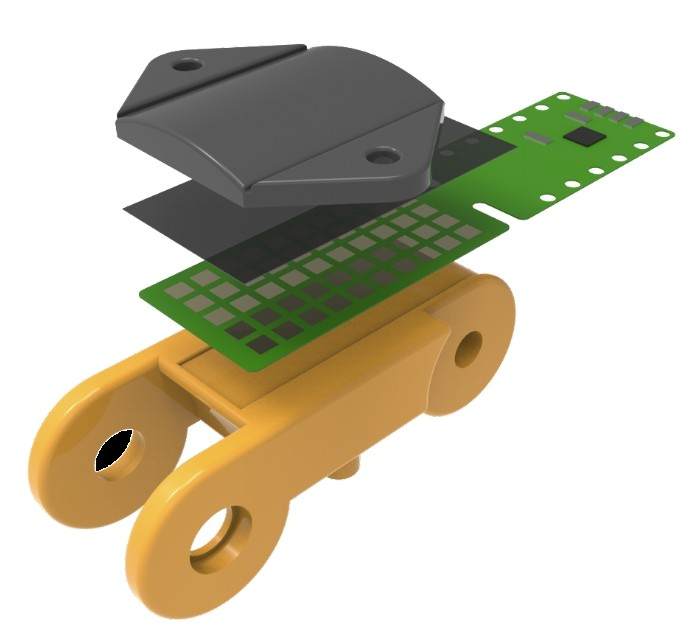
\includegraphics[width=0.5\textwidth]{figures/velostat-sensor.jpg}	
	\caption[Example of instrumenting the robot.]{Example of instrumenting a robot's finger with tactile sensors. A grid-like sensor array is attached to the finger and protected by silicone pads.}
	\label{fig:instrumentation_example}
\end{figure}

% instrument the OBJECT
A second location where instrumentation is applied is on the target object to manipulate itself. A prominent example is the instrumented Rubik's cube in \autocite{openai2019solving}. To avoid letting the robot learn to infer the Rubik's cube state from camera, they equip the cube with rotary encoders to track face rotations. In the deformable object manipulation domain, \Textcite{Bersch2011, Elbrechter2012} apply fiducial markers on cloth and paper for state estimation. However, visual markers suffer from occlusion and make it hard to generalize for other clothing articles without markers. Smart textiles, i.e.\ textiles that are able to sense stimuli from the environment and react accordingly \autocite{schnee17}, are being used in numerous applications such as health monitoring \autocite{Cochrane2019}, sports \autocite{Presti2019} and robotics \autocite{Yuen2017}. An example of textile with integrated eletronics is shown in \cref{fig:smart_textile_example}. Textile able to infer its own state is in particular interest for learning to manipulate clothing articles. To the best of our knowledge, there is no work of physical smart textiles for learning deformable object manipulation with robots. 

\begin{figure}[htbp]
	\centering
	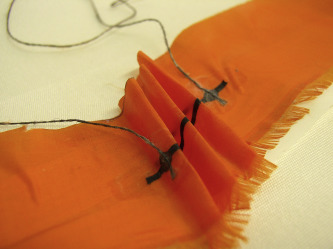
\includegraphics{figures/smart-textile-polymer.jpg}	
	\caption[Example of a smart textile implementation.]{Example of a smart textile implementation using a conductive polymer attached to the fabric. Figure from \autocite{Cochrane2019}.}
	\label{fig:smart_textile_example}
\end{figure}

% instrument the ENVIRONMENT
A final option on entities to instrumentify can be found in the environment itself. For example, a table can be equipped with force sensors that provide the location of objects to a robot. A concrete example can be found in \autocite{Kimura2013} who place a scale on the table with objects that have to be recognized and add the weight as input modality for control tasks. 
	
\section{Conclusion}

% geen meta inzichten
% de inhoud hiervan condenseren en een brug maken van h1 RO's naar rest van het boek (het werk dat zelf  gedaan is). 
% 	Data collection 	
%   Simulation
% 	Reward learning 
% 		SSL
% 	Instrumentation 
% 	

This chapter has reviewed, in a tutorial and survey style, the transition from traditional control pipelines for deformable object manipulation to leveraging learning methods. We have discussed methodologies, tools and approaches to building a cloth folding pipeline while identifying strenghts, weaknesses and gaps. 
One of those gaps is the state estimation of cloth in the modern deep learning era. We found that the majority of work employ vision for estimating the state of clothing articles. In our research, we step away from this vast focus on vision-only sensing and integrate tactile sensors in order to create a smart cloth that can tell a robot its state. 
We stressed the importance of simulation environments for robotic learning and the importance of realistic cloth simulation. We will examine a basic implementation and discuss its usefulness, Sim2Real pitfalls and application for learning to fold clothing.  
We highlighted the potential for example-based learning and learning from interaction using expressive representation methods in deep learning. In this research, we combine both approaches to exploit their strenghts: we use human demonstrations as examples for distilling task intent while letting the robot interact with the environment. To avoid expensive data labeling, we will introduce a self-supervised approach. 
We will start introducing our research in the next chapter that deals with addressing the problem that the prerequisite for learning is unavailable: gathering a high-quality, high-volume dataset of folding demonstrations. 

% \printbibliography

\end{document}